\documentclass[oneside,final,a4 paper]{hcmut-report}
\usepackage{tabularx,microtype,xurl,needspace}
\usepackage[section]{placeins}
\usepackage{tikz}
\usetikzlibrary{arrows.meta,positioning}
\setlength{\parindent}{0 pt}
\setlength{\emergencystretch}{3 em}
\setlength{\headheight}{44.3 pt}
\setlength{\tabcolsep}{4 pt}
\captionsetup{font=small,labelfont=bf}
\newcommand{\cls}[1]{\texttt{\detokenize{#1}}}
\newcolumntype{Y}{>{\raggedright\arraybackslash}X}
\makeatletter
\renewcommand\small{\@setfontsize\small{11 pt}{13.2 pt}}
\renewcommand\footnotesize{\@setfontsize\footnotesize{10 pt}{12 pt}}
\makeatother
\deptname{Faculty of Computer Science and Engineering}
\coursename{Deep Learning and Its Applications (CO3133)}
\reporttype{ASSIGNMENT 2 -- FINAL REPORT}
\title{Video-Disjoint Semantic Segmentation of Marine Debris in TrashCan}
\advisor{Dr. Le Thanh Sach}
\groupname{Tiki-taka}
\reportplace{Ho Chi Minh City}
\reporttime{8 November 2026}
\logofile{hcmut.png}
\hypersetup{pdftitle={Tiki-taka A2 Final: Video-Disjoint Semantic Segmentation},pdfauthor={Nguyen Anh Khoa; Nguyen Hao Thien; Ta Tuan Khai}}

\begin{document}
\hypersetup{pageanchor=false}
\thispagestyle{empty}
\begin{center}
{\bfseries\fontsize{14}{17}\selectfont VIETNAM NATIONAL UNIVERSITY, HO CHI MINH CITY\par
HO CHI MINH CITY UNIVERSITY OF TECHNOLOGY\par
FACULTY OF COMPUTER SCIENCE AND ENGINEERING\par}
\vspace{0.8 cm}

\includegraphics[width=3cm]{hcmut.png}\par
\vspace{0.6 cm}
{\bfseries\fontsize{17}{21}\selectfont DEEP LEARNING AND ITS APPLICATIONS\par}
{\bfseries CO3133 -- SEMESTER-261\par}
\vspace{0.5 cm}
{\bfseries\fontsize{16}{20}\selectfont ASSIGNMENT 2 -- FINAL REPORT\par}
\vspace{0.5 cm}
{\bfseries\fontsize{20}{24}\selectfont Video-Disjoint Semantic Segmentation\par of Marine Debris in TrashCan\par}
\vspace{0.4 cm}
{\large Video-disjoint evaluation of U-Net and SegFormer-B0\par}
\vspace{0.7 cm}
\begin{tabular}{rl}
\textbf{Class:} & CC01\\
\textbf{Instructor:} & Dr. Le Thanh Sach\\
\textbf{Group:} & Tiki-taka\\
\textbf{Milestone:} & Final\\
\textbf{Evidence cutoff:} & 8 November 2026
\end{tabular}\par
\vspace{0.5 cm}
\begin{tabular}{clc}\toprule
No. & Group member & Student ID\\\midrule
1 & Nguyen Anh Khoa & 2452539\\
2 & Nguyen Hao Thien & 2453194\\
3 & Ta Tuan Khai & 2452515\\\bottomrule
\end{tabular}
\vfill
{\bfseries Ho Chi Minh City, 8 November 2026}
\end{center}
\clearpage
\hypersetup{pageanchor=true}
\pagenumbering{roman}
\section*{Abstract}
\addcontentsline{toc}{section}{Abstract}
We compare scratch U-Net and two pretrained SegFormer-B0 configurations on a video-disjoint TrashCan-Material split. The SegFormer configurations differ in training color augmentation. We report nine runs over three seeds on the same 1,078 held-out images.

Mean test foreground mean intersection over union (mIoU) is 4.52\% for U-Net, 15.86\% for SegFormer without augmentation and 15.41\% for SegFormer with augmentation. Both SegFormer configurations exceed U-Net at each measured seed. The augmentation difference changes sign across seeds. The augmented model assigns more true trash pixels to background at each seed. Matched qualitative cases show thin-object recovery, foreground omissions and material confusion.

We report inference cost under one T4 batch protocol and keep the seed-level outcomes visible. The results describe one fixed split and recorded Kaggle and Colab execution profiles.

\vspace{0.4 cm}
\textbf{Keywords:} semantic segmentation, marine debris, TrashCan, U-Net, SegFormer, video-disjoint evaluation.
\clearpage
\begingroup
\setstretch{1.0}
\tableofcontents
\endgroup
\clearpage
\pagenumbering{arabic}
\section{Problem and data description}
\subsection{Task and research objectives}
Underwater debris is difficult to distinguish from marine life and the seafloor because object appearance, scale, illumination and occlusion vary. TrashCan supplies underwater images with object-level annotations for marine debris research\cite{trashcan}. This project converts the polygons into a semantic segmentation task: each valid image pixel receives one class label, without distinguishing separate instances of the same class.

For an RGB image $x\in\mathbb{R}^{H\times W\times 3}$, the model predicts a map $\hat y\in\{0,\ldots,16\}^{H\times W}$. There are \textbf{17 output classes: background plus 16 foreground categories}. The foreground comprises ROV, plant, six animal categories and eight trash categories. Ignore label 255 is excluded from supervision and evaluation.

An underwater image may contain several objects and classes. The task requires the model to locate their boundaries and assign a category at each pixel. Two pieces of plastic receive the same class ID. The remotely operated vehicle (ROV) and marine life are foreground categories alongside trash. Padding and ambiguous cross-class overlap are excluded through the ignore label.

The project asks three questions.
\begin{enumerate}
\item Under a fixed video-disjoint split, how do a scratch U-Net and a pretrained SegFormer-B0 compare on foreground and trash overlap? The comparison includes each configuration's architecture, initialization and learning rate.
\item With the SegFormer architecture and starting weights matched by seed, does mild training RGB color jitter improve trash overlap while preserving foreground quality? The proposal criterion is at least a 1-point gain in validation trash mIoU, with at most a 1-point loss in each of validation foreground mIoU and Dice.
\item What types of errors persist, and what does each configuration cost to run? We use pixel-level class confusions, aligned test predictions and recorded forward latency under one matched Tesla T4 protocol.
\end{enumerate}
The practical work covers polygon-to-mask conversion, splitting by video, a shared training and evaluation engine, nine model--seed runs, and verification of saved results. The criterion in Question 2 is a predeclared validation target. The held-out evaluation tests the selected checkpoints independently of that criterion.

\subsection{Dataset source and provenance}
The working dataset is TrashCan 1.0 Material. The exploratory data analysis (EDA), measured on 5 October 2026, records 7,212 RGB images,12,336 polygon annotations and 312 filename-derived video groups. There are 3,245 images at $480\times 360$ and 3,967 at $480\times 270$. Source imagery is credited to JAMSTEC and the dataset to Hong, Fulton and Sattar\cite{trashcan}.

The archive README credits the dataset authors and asks users to cite the TrashCan paper. Both annotation JSON files list an Attribution-NonCommercial-ShareAlike entry. The example figures use credited frames from the Material version. The report source package contains figures and manifests, with the dataset archive and checkpoint binaries kept separately.

The instructor approved the proposal according to the project owner's confirmation on 26 October 2026. This statement records the confirmation used by the training setup; it is not an independently inspected learning-management-system submission record.

\subsection{Video-disjoint partition and class support}
The original source partitions contain 6,008 training images and 1,204 validation images. They share 127 filename-derived video IDs. Separating individual frames using those source labels would therefore allow frames from the same video into different evaluation partitions.

The project instead uses a fixed seed 36 manifest that assigns each video to exactly one partition. Metadata-based split construction uses deterministic greedy/local-search candidates, with at least three supporting training videos and two supporting videos in each held-out partition per foreground class. Table~\ref{tab:split} records the resulting image, video and annotation counts. Pairwise video-ID overlap is zero.
\begin{table}[H]
\centering\small
\caption{Fixed video-disjoint partition, split seed 36. Native mask percentages are retained from the 5 October 2026 EDA.}\label{tab:split}
\begin{tabular}{lrrrrr}\toprule
Partition & Images & Videos & Annotations & Background (\%) & Ignore (\%) \\ \midrule
Train & 5,057 & 207 & 8,563 & 89.13 & 0.0371 \\
Validation & 1,077 & 54 & 1,956 & 89.34 & 0.0754 \\
Test & 1,078 & 51 & 1,817 & 90.33 & 0.0238 \\
\bottomrule\end{tabular}
\end{table}

Video grouping addresses frame-level overlap under the chosen ID convention. It does not prove independence of dive locations or visually related scenes carrying different video IDs.

Class imbalance remains substantial after splitting. Table~\ref{tab:support} gives each foreground class's annotation count, video support and native supervised pixel totals. The small support for categories such as animal shells makes macro overlap and per-class results more informative than background-dominated accuracy.
\begin{table}[H]
\centering\small
\caption{Foreground class support in the fixed split. Pixel counts are native-resolution supervised pixels in millions, before letterboxing.}\label{tab:support}
\begin{tabular}{lrrrrrrr}\toprule
Class & Ann. & \multicolumn{3}{c}{Videos (train/val/test)} & \multicolumn{3}{c}{Pixels, M (train/val/test)} \\ \midrule
\cls{rov} & 3317 & 99 & 22 & 24 & 39.554 & 7.164 & 6.736 \\
\cls{plant} & 507 & 17 & 10 & 5 & 2.363 & 0.586 & 0.661 \\
\cls{animal_fish} & 764 & 33 & 7 & 5 & 4.421 & 1.444 & 1.577 \\
\cls{animal_starfish} & 398 & 9 & 3 & 3 & 0.123 & 0.037 & 0.022 \\
\cls{animal_shells} & 249 & 3 & 2 & 2 & 0.104 & 0.087 & 0.006 \\
\cls{animal_crab} & 309 & 9 & 3 & 3 & 0.789 & 0.199 & 0.196 \\
\cls{animal_eel} & 343 & 24 & 6 & 5 & 0.255 & 0.057 & 0.076 \\
\cls{animal_etc} & 235 & 12 & 6 & 7 & 0.805 & 0.079 & 0.177 \\
\cls{trash_etc} & 2039 & 107 & 23 & 23 & 9.145 & 1.921 & 1.601 \\
\cls{trash_fabric} & 314 & 14 & 4 & 3 & 2.285 & 0.422 & 0.352 \\
\cls{trash_fishing_gear} & 196 & 10 & 2 & 2 & 1.465 & 0.328 & 0.215 \\
\cls{trash_metal} & 1126 & 42 & 12 & 8 & 3.590 & 0.638 & 1.275 \\
\cls{trash_paper} & 193 & 6 & 2 & 2 & 0.947 & 0.257 & 0.056 \\
\cls{trash_plastic} & 1864 & 61 & 16 & 20 & 12.865 & 2.535 & 2.480 \\
\cls{trash_rubber} & 142 & 3 & 2 & 2 & 0.203 & 0.243 & 0.047 \\
\cls{trash_wood} & 340 & 14 & 3 & 3 & 2.900 & 0.467 & 0.332 \\
\bottomrule\end{tabular}
\end{table}

These counts describe dense native masks before resizing; they must not be mixed with the 512-canvas pixel totals reported by the evaluator.

The retained EDA figures provide a visual summary of the same imbalance and group coverage. Figure~\ref{fig:distribution} shows category frequencies, and Figure~\ref{fig:videos} shows support across video groups. Counts are from the 5 October audit rather than a new raw-data measurement in this report update.
\begin{figure}[H]\centering
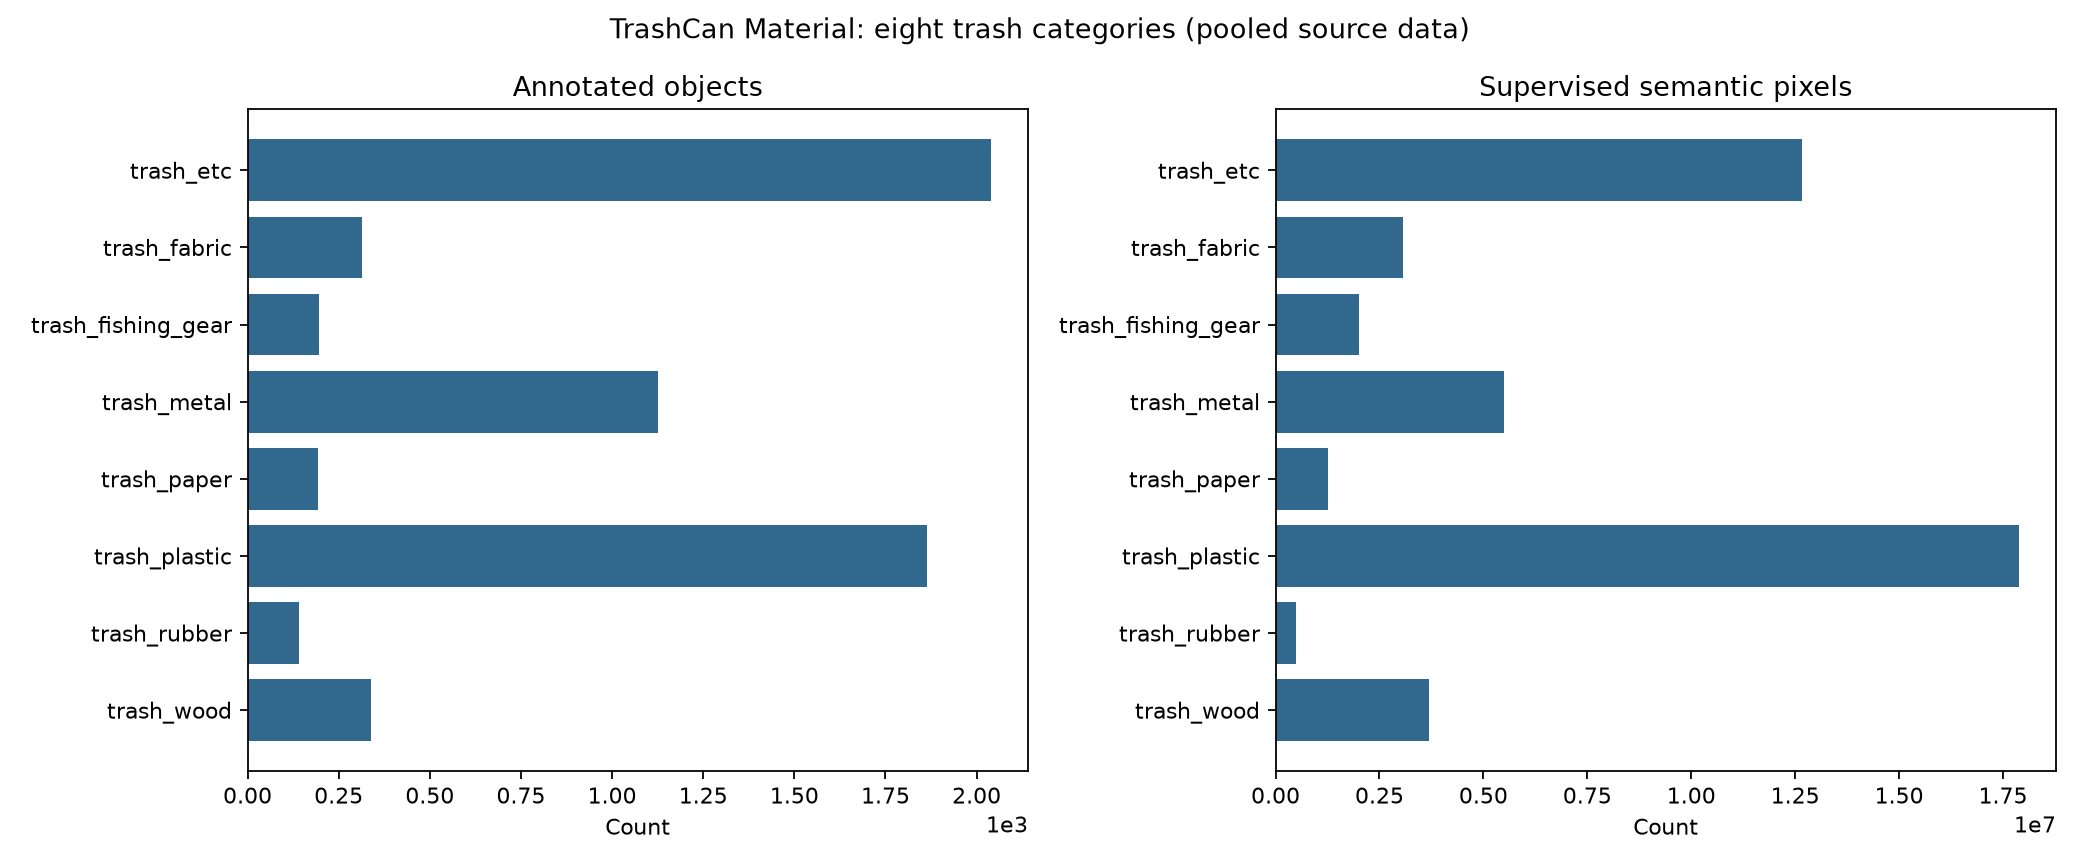
\includegraphics[width=.94\textwidth]{images/material_distribution.png}
\caption{Material-category distribution from the retained EDA.}\label{fig:distribution}
\end{figure}
\begin{figure}[H]\centering
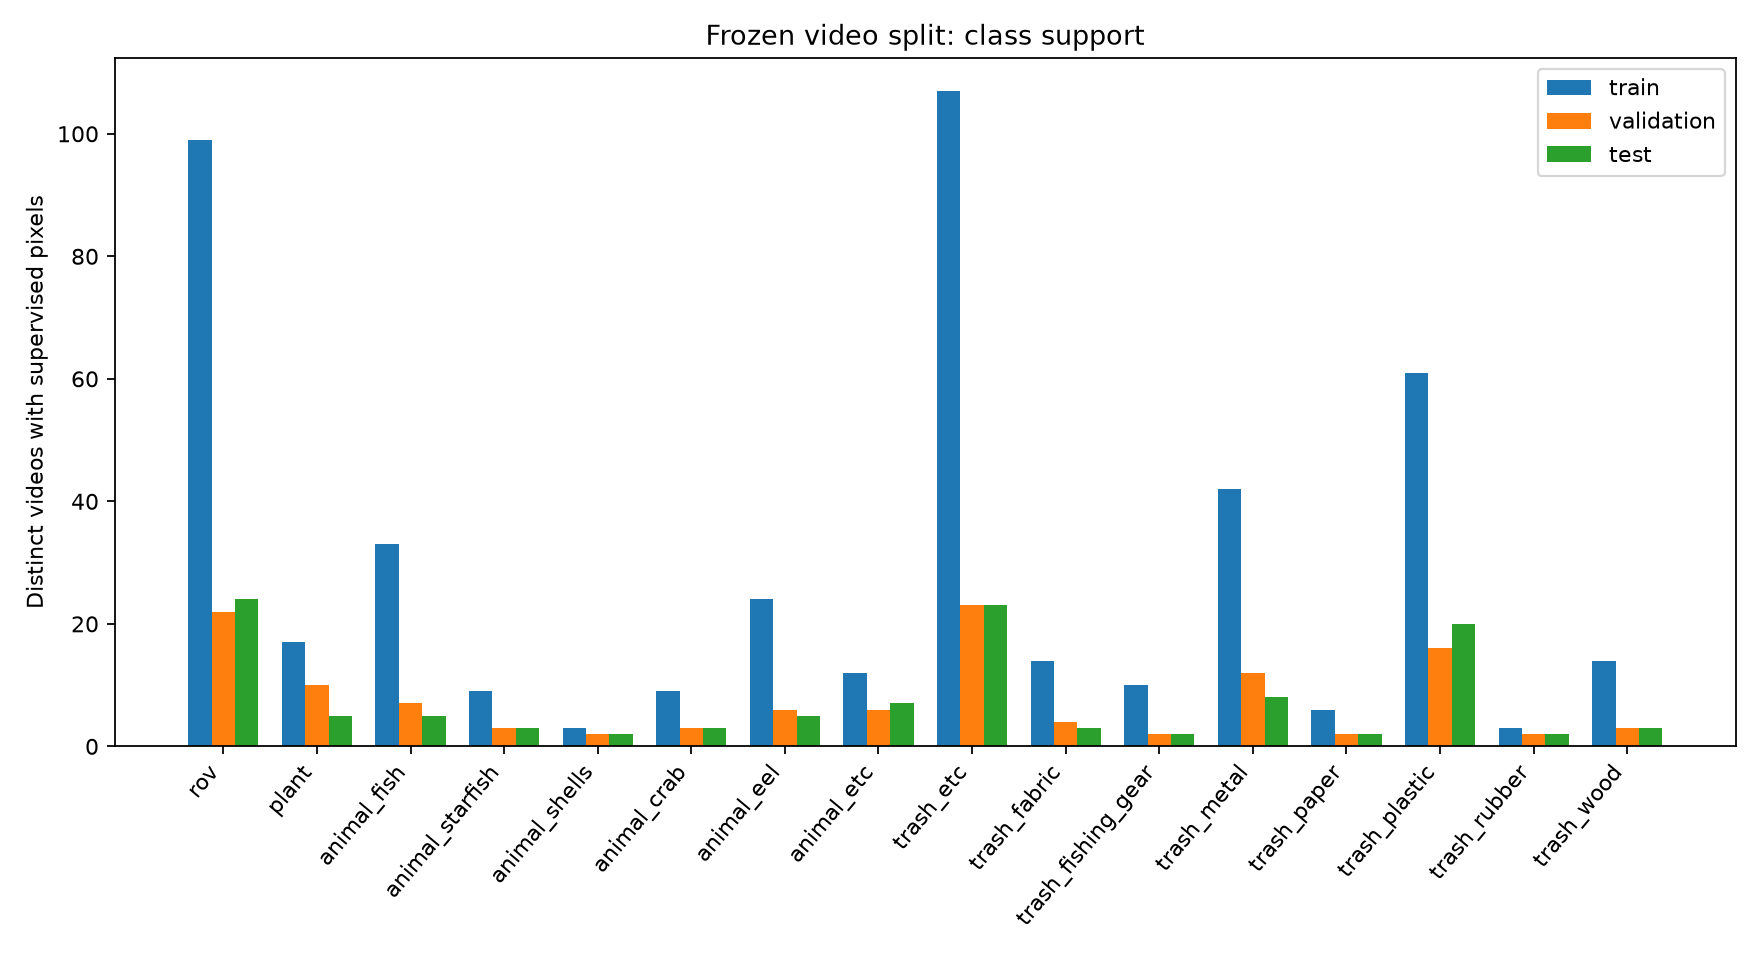
\includegraphics[width=.94\textwidth]{images/split_class_video_support.png}
\caption{Per-class video support under the fixed seed 36 split.}\label{fig:videos}
\end{figure}
The split provides class coverage in every partition while retaining rare classes; it does not remove their statistical uncertainty.

\clearpage
\subsection{Mask conversion, preprocessing and checks}
Polygons are rasterized on the native image canvas with Pillow 12.3.0. Same-class polygons are unioned; pixels where different foreground classes overlap receive ignore 255. Out-of-canvas regions are clipped. The EDA found no annotation that rasterized to an empty mask under this converter.

Each image is letterboxed to $512\times 512$ while preserving aspect ratio. RGB uses bilinear resizing, masks use nearest-neighbor resizing, RGB padding is black and target padding is ignore 255. The tensor is normalized with ImageNet channel means $(0.485,0.456,0.406)$ and standard deviations $(0.229,0.224,0.225)$. There is no label reduction or second image-processor resize.

The training adapter checks the published manifest digest, source annotation hashes, image dimensions, membership and native target hash. The supplied checks cover 5,057 training and 1,077 validation images. Figure~\ref{fig:qa} reproduces existing EDA annotation checks; it is not a gallery of model predictions.
At evaluation resolution, ignored pixels include the much larger letterbox padding region as well as native annotation conflicts. For example, U-Net test ignore fraction is 34.06\%; this does not mean that 34.06\% of the native annotations are conflicting.
\begin{figure}[H]\centering
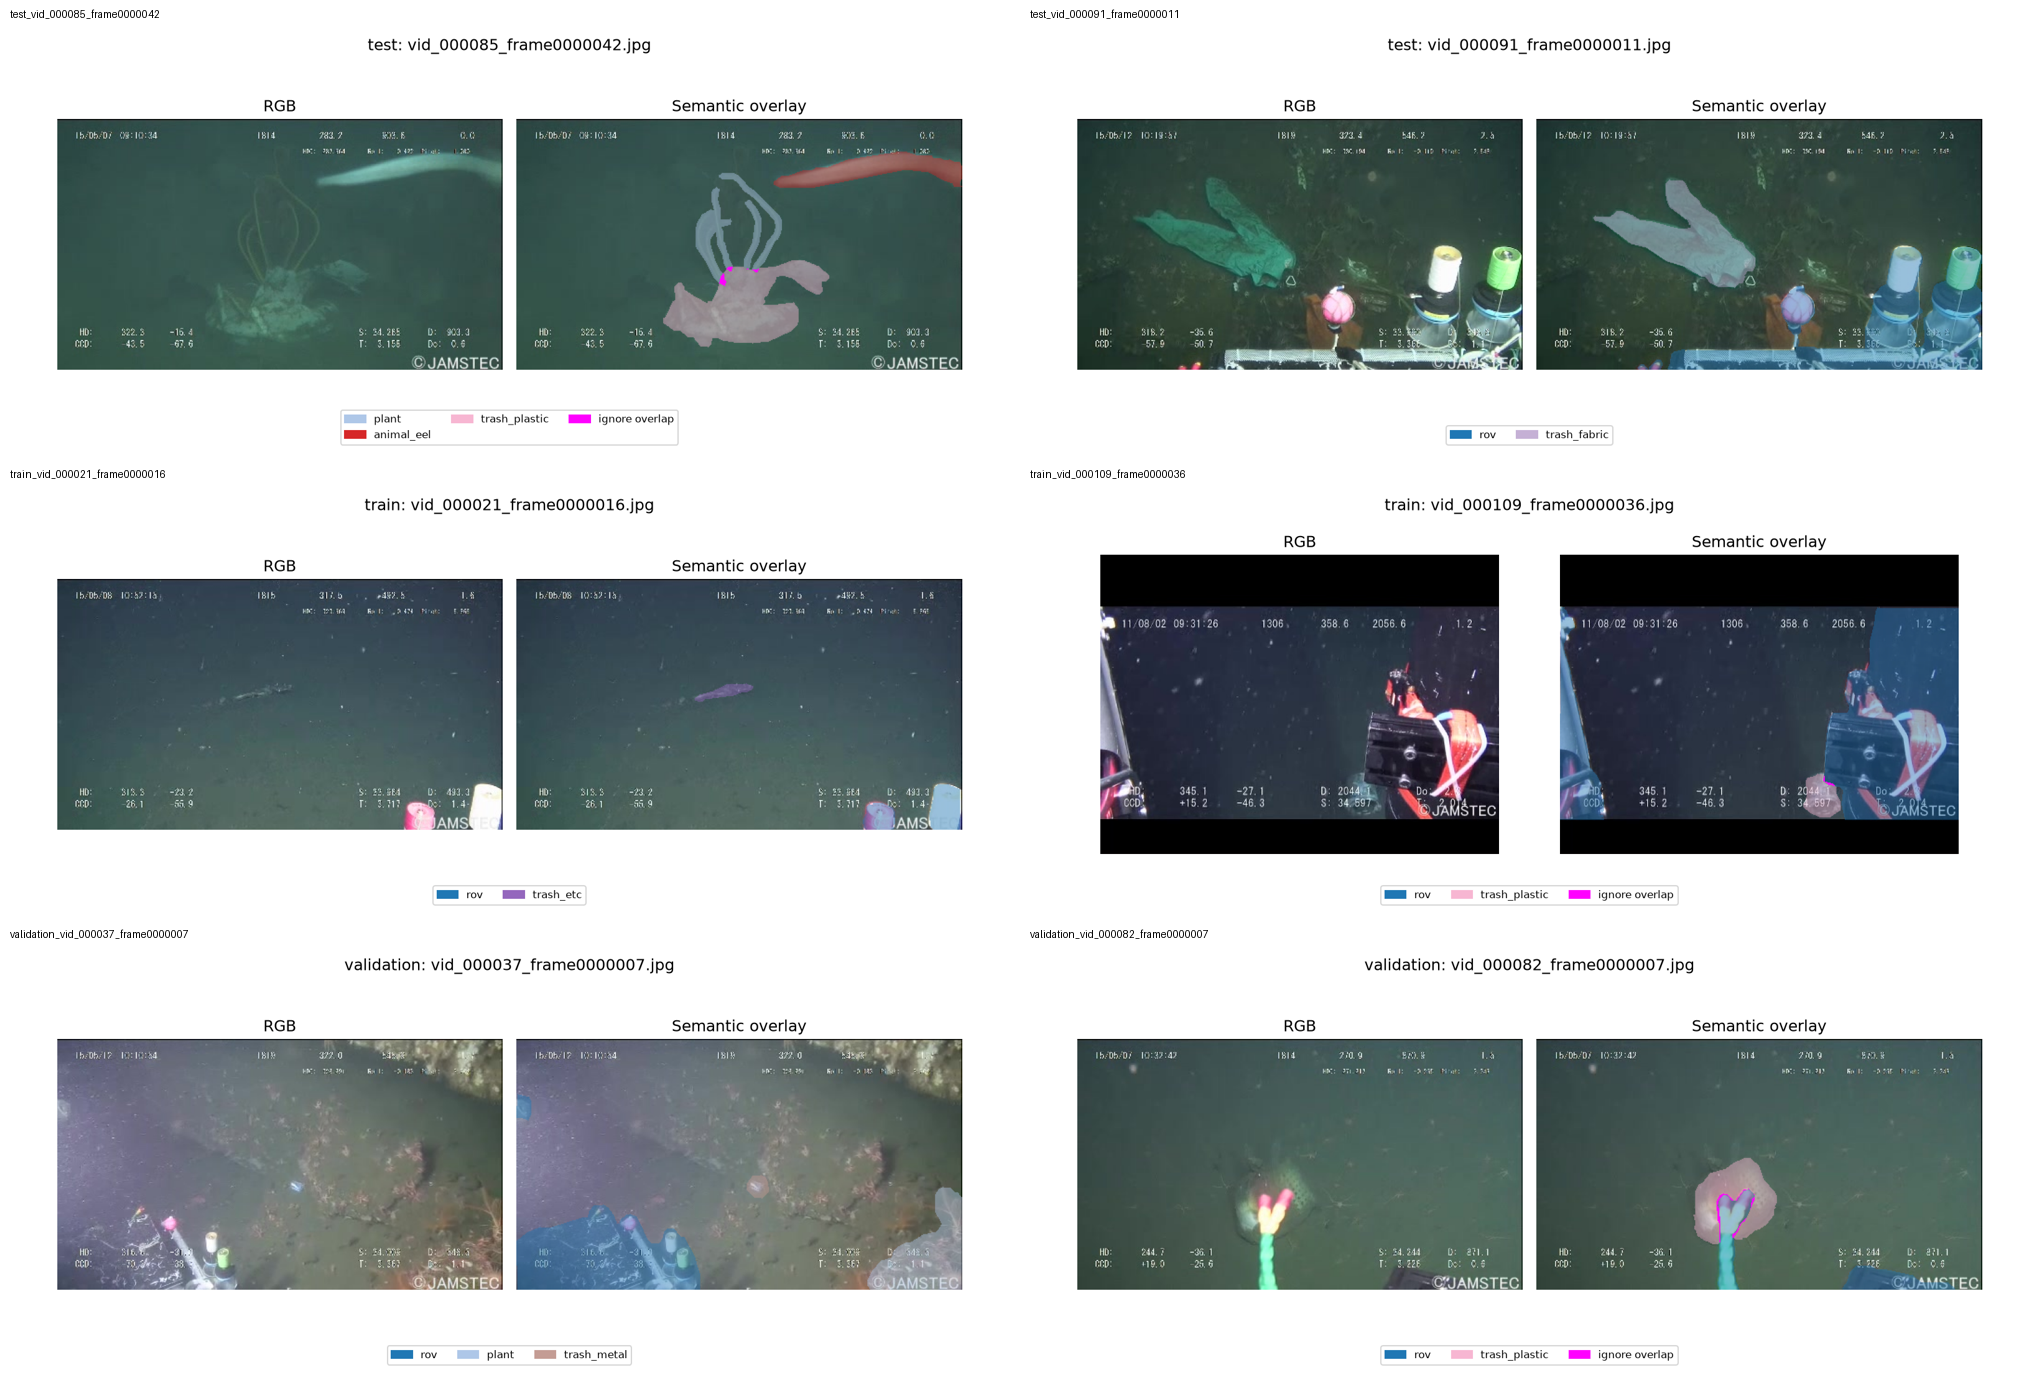
\includegraphics[width=.80\textwidth]{images/annotation_qa.png}
\caption{Six retained native annotation-QA examples, two per partition. RGB/mask overlays check conversion and alignment; they are ground truth, not inference outputs.}\label{fig:qa}
\end{figure}

\clearpage
\subsection{Example training batch and color augmentation}
Figure~\ref{fig:batch} recreates the first shuffled training batch of epoch 1 for seed 69 with the saved manifest, frozen preprocessing and original data loader. The input tensor is $4\times3\times512\times512$ in channel-first order. The integer target tensor is $4\times512\times512$ and stores one class ID per pixel. Displayed RGB reverses channel normalization.

\begin{figure}[H]\centering
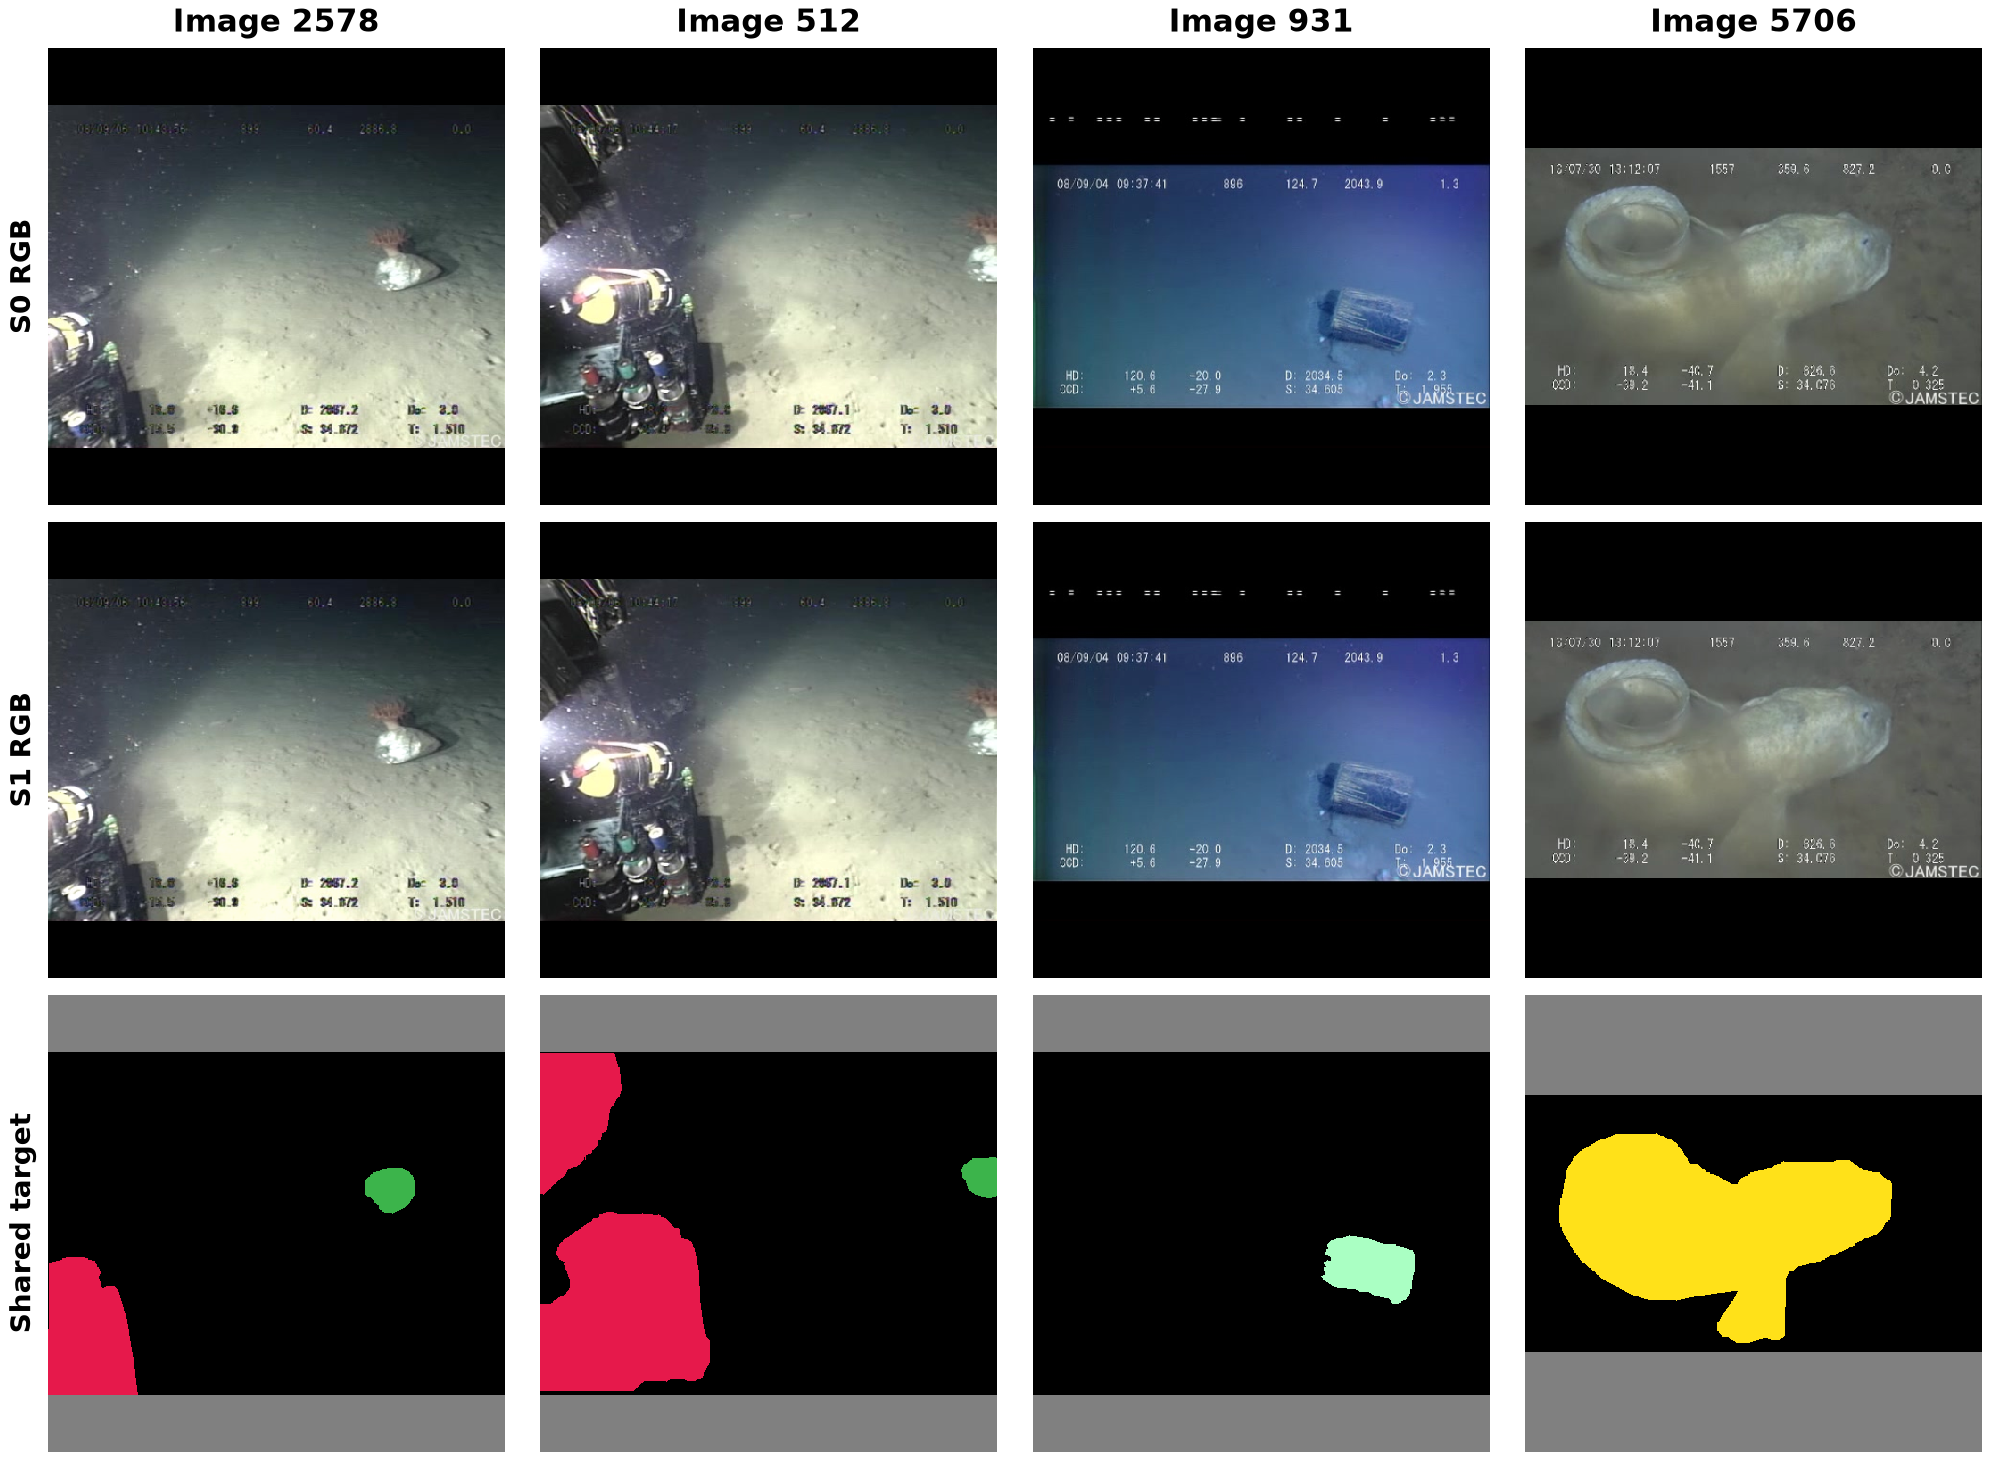
\includegraphics[width=.97\textwidth]{images/a2_training_batch.png}
\caption{Regenerated training batch with S0 RGB, S1 RGB and shared semantic targets. Gray is ignore 255, black is background, red is ROV, green is plant, pale green is wood and yellow is fish. Source imagery is from JAMSTEC via TrashCan-Material.}\label{fig:batch}
\end{figure}

The S1 color operation changes RGB for images 2578, 931 and 5706 in this batch. Image 512 takes the identity branch. All four masks match exactly between S0 and S1, including the wood target in image 931 and the fish target in image 5706. The figure is a replay of the data loader on CPU. The evidence package records the IDs and target hashes in \path{evidence/example_batch.json}.

\clearpage
\section{Methodology}
\subsection{Implemented pipeline}
The common pipeline keeps data conversion, objective and scoring consistent across models. Figure~\ref{fig:pipeline} shows the main flow; test data enters only the final evaluation stage of a completed run.
\begin{figure}[H]\centering
\begin{tikzpicture}[node distance=4 mm,box/.style={draw,rounded corners,align=center,text width=25 mm,minimum height=16 mm,font=\small},>=Latex]
\node[box](a){RGB and\linebreak polygons};
\node[box,right=of a](b){Rasterize;\linebreak video split};
\node[box,right=of b](c){Letterbox;\linebreak normalize};
\node[box,right=of c](d){U-Net or\linebreak SegFormer};
\node[box,right=of d](e){Train CE+Dice;\linebreak validate};
\node[box,below=7 mm of e](f){Select best;\linebreak evaluate test};
\draw[->](a)--(b);\draw[->](b)--(c);\draw[->](c)--(d);\draw[->](d)--(e);\draw[->](e)--(f);
\end{tikzpicture}
\caption{Shared segmentation workflow. Test scores do not select the training epoch.}\label{fig:pipeline}
\end{figure}
This separation makes the S0/S1 experiment a change to training RGB color augmentation while preserving the mask and evaluation conventions.

\subsection{Segmentation theory and tensor interface}
Each model maps $B\times3\times H\times W$ RGB inputs to aligned $B\times17\times H\times W$ logits. A logit is an unnormalized class score. The softmax across the 17 channels gives a probability distribution at each location, and the largest logit determines the discrete predicted label. In this experiment $H=W=512$. The mask tensor contains integer labels at the same spatial coordinates. Pixels with label 255 contribute to neither loss nor the confusion matrix.

A small piece of debris can occupy only a few pixels while most of the image shows the seafloor. Strided encoding increases the context available to classify the small region but reduces its spatial resolution. U-Net restores detail through high-resolution encoder skips. SegFormer fuses four feature scales that capture different amounts of context. Both decoders align their predictions to the input canvas.

\clearpage
\subsection{Scratch U-Net baseline}
The compact U-Net follows an encoder--decoder design with skip connections\cite{unet}. The implemented version has four downsampling stages and channel widths 16,32,64,128,256. Each block contains two bias-free $3\times 3$ convolutions, eight-group Group Normalization and ReLU. Downsampling uses $2\times 2$ max pooling. The decoder upsamples bilinearly with \cls{align_corners=false}, concatenates encoder features, and applies another two-convolution block. A $1\times 1$ head produces 17 logits per pixel.

All 1,964,369 parameter elements are trainable, with zero frozen parameters. The model is initialized from scratch. The scratch configuration supplies the architecture baseline.

At each decoder level, the upsampled feature and the same-resolution encoder feature are concatenated channel-wise. The encoder path therefore carries local texture and boundaries around the low-resolution bottleneck. The stages of the implemented network are shown in Figure~\ref{fig:models}.

\subsection{Pretrained SegFormer-B0 and full fine-tuning}
SegFormer combines a hierarchical Transformer encoder with a lightweight multilayer-perceptron decoder\cite{segformer}. The implementation loads \path{nvidia/segformer-b0-finetuned-ade-512-512}, pinned to revision \path{489d5cd81a0b59fab9b7ea758d3548ebe99677da}. The pretrained encoder and compatible decoder weights are retained, while the 150-class ADE20K classifier is replaced by a newly initialized 17-class classifier.

The complete model is fine-tuned end to end: encoder, decoder and classifier parameters all receive updates. Total and trainable counts are both 3,718,513; frozen count is zero. Pretrained initialization therefore does not imply a frozen backbone. Lower-resolution raw logits are bilinearly interpolated to the 512-canvas target before computing loss and argmax predictions.

The main-run initial-state hashes match between S0 and S1 within each of the three matched run seeds.

The Mix Transformer B0 encoder uses overlapping patch projections at successive spatial strides and outputs four feature maps at resolutions $1/4$, $1/8$, $1/16$ and $1/32$ of the input. Self-attention mixes information between locations. Spatial reduction of keys and values reduces its cost at the larger resolutions. The decoder projects each scale to width 256, upsamples to the $1/4$ grid, concatenates and fuses the features, then applies the 17-class head. The pinned architecture configuration specifies channel widths 32, 64, 160 and 256 and two blocks per stage\cite{segformerconfig}.

\clearpage
\begingroup
\setstretch{1.05}
\setlength{\intextsep}{7pt}
\begin{figure}[H]\centering
\scalebox{.84}{\begin{tikzpicture}[x=1cm,y=1cm,>=Latex,
  block/.style={draw,rounded corners=2pt,minimum width=2.38cm,minimum height=.60cm,align=center,font=\footnotesize},
  enc/.style={block,fill=blue!6},dec/.style={block,fill=teal!9},logits/.style={block,fill=black!6}]
\node[anchor=west,font=\bfseries] at (-1.18,1.0) {U-Net (scratch)};
\foreach \col/\dim/\chan in {0/512/16,1/256/32,2/128/64,3/64/128,4/32/256} {
  \node[enc] (u\col) at (\col*2.63,0) {$\dim^2\!\times\!\chan$};
}
\foreach \src/\dst in {0/1,1/2,2/3,3/4} {\draw[->] (u\src)--(u\dst);}
\foreach \col/\dim/\chan in {0/512/16,1/256/32,2/128/64,3/64/128} {
  \node[dec] (d\col) at (\col*2.63,-1.02) {$\dim^2\!\times\!\chan$};
  \draw[->,dashed,gray] (u\col)--(d\col);
}
\foreach \src/\dst in {1/0,2/1,3/2} {\draw[->] (d\src)--(d\dst);}
\draw[->] (u4.south) |- (d3.east);
\node[logits] (uhead) at (0,-2.03) {$512^2\!\times\!17$};
\draw[->] (d0)--(uhead);
\node[anchor=west,font=\footnotesize] at (1.42,-2.03)
  {Max pooling $\rightarrow$ bottleneck $\rightarrow$ bilinear upsampling and skips};

\node[anchor=west,font=\bfseries] at (-1.18,-3.03) {SegFormer-B0 (pretrained)};
\foreach \col/\dim/\chan in {0/128/32,1/64/64,2/32/160,3/16/256} {
  \node[enc] (s\col) at (\col*2.63,-3.91) {$\dim^2\!\times\!\chan$};
}
\foreach \src/\dst in {0/1,1/2,2/3} {\draw[->] (s\src)--(s\dst);}
\node[dec,minimum width=6cm] (fuse) at (3.94,-5.0) {Project, align and fuse at $128^2$};
\foreach \col/\stop in {0/1.5,1/2.63,2/5.26,3/6.4} {
  \draw[->] (s\col.south) -- ++(0,-.18) -| (\stop,-4.70);
}
\node[logits] (head) at (8.50,-5.0) {$128^2\!\times\!17$};
\node[logits] (aligned) at (11.26,-5.0) {$512^2\!\times\!17$};
\draw[->] (fuse)--(head);
\draw[->] (head)--(aligned);
\end{tikzpicture}
}
\caption{Implemented U-Net and SegFormer-B0 feature paths. Each box lists spatial size and channel count for a $512\times512$ input. Dashed U-Net paths are skip connections. SegFormer projects and aligns all four feature scales before fusion.}\label{fig:models}
\end{figure}
The two paths meet the same full-resolution logit interface.

\subsection{Objective and evaluation metrics}
Training minimizes the sum of multiclass cross-entropy and foreground soft Dice loss, each with coefficient 1:
\begin{equation}
\mathcal L=\mathcal L_{\mathrm{CE}}+\frac{1}{|C_B|}\sum_{c\in C_B}\left(1-\frac{2\sum_{i\in V_B}p_{ic}y_{ic}+\epsilon}{\sum_{i\in V_B}(p_{ic}+y_{ic})+\epsilon}\right).
\end{equation}
Here $V_B$ is the set of valid pixels in a batch, $C_B$ contains foreground classes present in the target, $p_{ic}$ is the softmax probability, $y_{ic}$ is the one-hot target and $\epsilon=10^{-6}$. A batch with no foreground contributes zero Dice loss. The optimizer skips all-ignore batches. The logged epoch loss averages batch objectives weighted by valid pixel count.

Cross-entropy penalizes low probability on the correct class at each valid pixel. Soft Dice gives equal weight to each present foreground class. A model can reduce cross-entropy across a large seafloor region while still missing a small piece of debris. Dice penalizes that omission for the debris class.

For hard predictions, the evaluator accumulates one 17-by 17 confusion matrix across the whole partition. For class $c$,
\begin{equation}
\operatorname{IoU}_c=\frac{TP_c}{TP_c+FP_c+FN_c},\qquad
\operatorname{Dice}_c=\frac{2TP_c}{2TP_c+FP_c+FN_c}.
\end{equation}
Rows are ground truth and columns are predictions. Foreground metrics average IDs 1--16. Trash mIoU averages IDs 9--16. All foreground classes have defined IoU on test. Pixel accuracy is the diagonal sum divided by valid pixels.

\par
\endgroup
\clearpage
\subsection{Training budget, checkpointing and environment}
Both model families use AdamW, weight decay 0.01, batch 4, up to 40 epochs, patience 8, FP 32, no learning-rate scheduler and no mixed precision. U-Net learning rate is $10^{-3}$; SegFormer uses $6\times 10^{-5}$. Training seeds 69420, 67 and 69 are distinct from split seed 36. The training loader shuffles with a separate generator seeded by run seed plus epoch; validation/test are unshuffled.

The best checkpoint maximizes validation foreground mIoU; a tie uses lower validation loss, then the earlier epoch. Each completed epoch saves model, AdamW state, random-number states, history, best selection and early-stopping counter. Resume restores this state; an incomplete epoch is repeated. The U-Net continuation belongs to the same experiment and is not an independent seed.

The supplied runs/pilots record a Tesla T4 with 14.56 GiB memory, Python 3.13.16, PyTorch 2.11.0+cu 130, torchvision 0.26.0+cu 130 and NumPy 2.1.3. Pillow 12.3.0 and Transformers 4.57.6 are pinned. TF 32 is disabled and CUDA deterministic algorithms use warning-only mode for the bilinear-backward limitation. These settings and saved RNG state do not promise cross-runtime GPU bitwise identity.

\subsection{Color augmentation and execution profiles}
S0 disables color jitter. S1 applies it to training RGB with probability 0.5: brightness, contrast and saturation factors are sampled in $[0.9,1.1]$, hue shift in $[-0.01,0.01]$, with shuffled operation order. Masks are unchanged. A seed/epoch/image-specific random stream keeps augmentation separate from model and sampling randomness. There is no geometric augmentation; held-out images are unaugmented.

The paired configurations share architecture, pretrained revision, seed, split, normalization, optimizer, learning rate, loss and budget. The intended treatment is the training RGB color switch. Table~\ref{tab:final-seed-results} records actual execution profiles. S0 at seed 67 resumed on Colab from a Kaggle checkpoint after seven epochs. This continuation preserves the seed and training history.

Underwater lighting and camera conditions can change apparent color and contrast. The experiment tests whether mild photometric variation helps robustness while preserving the spatial target. Color can also help distinguish materials, so the effect on trash categories is empirical. Figure~\ref{fig:batch} shows the actual transform branches. The S0/S1 comparison controls the initial state and nominal training protocol. The U/S0 comparison also changes initialization, parameter count and learning rate.

\clearpage
\section{Results}
\subsection{Held-out scores by model and seed}
Table~\ref{tab:final-seed-results} reports all nine test runs on the same 1,078 held-out images. Foreground (FG) scores average the 16 non-background classes, while trash mIoU averages the eight trash classes. U denotes scratch U-Net. S0 and S1 are pretrained SegFormer-B0 with training color augmentation off and on. Checkpoints are selected on validation using FG mIoU, then validation loss and earlier epoch as tie-breakers.

\begin{table}[H]\centering\small
\caption{Held-out scores by model and seed. Epochs are final/selected.}\label{tab:final-seed-results}
\begin{tabular}{@{}rllrrrr@{}}\toprule
Seed & Run & Platform & Epochs & FG mIoU (\%) & FG Dice (\%) & Trash mIoU (\%) \\\midrule
69420 & U & Colab & 23/15 & 3.563 & 5.852 & 1.465 \\
69420 & S0 & Colab & 23/15 & 13.588 & 20.566 & 6.403 \\
69420 & S1 & Colab & 22/14 & 13.964 & 20.895 & 6.078 \\
67 & U & Kaggle & 23/15 & 4.901 & 7.911 & 1.915 \\
67 & S0 & Kaggle $\to$ Colab & 28/20 & 18.492 & 25.868 & 8.172 \\
67 & S1 & Colab & 17/9 & 17.621 & 25.158 & 5.596 \\
69 & U & Colab & 20/12 & 5.095 & 7.986 & 2.002 \\
69 & S0 & Colab & 16/8 & 15.489 & 21.993 & 5.217 \\
69 & S1 & Colab & 30/22 & 14.656 & 21.873 & 5.964 \\
\bottomrule
\end{tabular}
\end{table}

Table~\ref{tab:final-aggregate} summarizes the measured repeats. Both SegFormer configurations exceed the U-Net baseline on test foreground and trash mIoU at each seed. Architecture, initialization and learning rate differ, so this is a configuration-level comparison. Sample standard deviations are descriptive because there are only three repeats and the platforms vary across runs.

\begin{table}[H]\centering\small
\caption{Descriptive mean and sample standard deviation over three run seeds, in percent.}\label{tab:final-aggregate}
\begin{tabular}{@{}lrrr@{}}\toprule
Run & FG mIoU & FG Dice & Trash mIoU \\\midrule
U & $4.52 \pm 0.83$ & $7.25 \pm 1.21$ & $1.79 \pm 0.29$ \\
S0 & $15.86 \pm 2.47$ & $22.81 \pm 2.74$ & $6.60 \pm 1.49$ \\
S1 & $15.41 \pm 1.94$ & $22.64 \pm 2.23$ & $5.88 \pm 0.25$ \\
\bottomrule
\end{tabular}
\end{table}

\Needspace{17\baselineskip}
\subsection{Effect of color augmentation}
The hypothesis is that training color jitter improves trash overlap while preserving foreground quality. Within a seed the configurations share data, initial weights, model and optimization settings. The proposal rule requires validation trash mIoU to rise by at least 1 percentage point while validation FG mIoU and Dice each decline by no more than 1 point. Only seed 69 meets the rule. S0 at seed 67 includes a Kaggle-to-Colab continuation, so its paired result also has a runtime difference.

\begin{table}[H]\centering\small
\caption{S1 minus S0 on test, in percentage points. The last column applies the proposal rule to validation.}\label{tab:final-paired-deltas}
\begin{tabular}{@{}rrrrl@{}}\toprule
Seed & FG mIoU & FG Dice & Trash mIoU & Validation rule \\\midrule
69420 & +0.376 & +0.330 & -0.326 & Not met \\
67 & -0.870 & -0.709 & -2.576 & Not met \\
69 & -0.833 & -0.120 & +0.747 & Met \\
\bottomrule
\end{tabular}
\end{table}

Table~\ref{tab:final-paired-deltas} reports held-out outcomes separately from that validation rule. Test FG mIoU rises at seed 69420 and falls at seeds 67 and 69. Test trash mIoU rises only at seed 69. The observed changes support a seed-dependent trade-off, with limited evidence for a general improvement from this augmentation setting.

The analytical background-only reference in Table~\ref{tab:background} obtains about 90.35\% pixel accuracy with zero foreground overlap. This illustrates why foreground macro scores are more informative on this dataset.
\begin{table}[H]
\centering\small
\caption{Analytical constant-background reference derived from existing confusion-row supports; no model inference is required.}\label{tab:background}
\begin{tabular}{lrrrr}\toprule
Partition / predictor & Pixel acc. & FG mIoU & FG Dice & All mIoU \\ \midrule
Validation / background & 0.894015 & 0.000000 & 0.000000 & 0.052589 \\
Test / background & 0.903466 & 0.000000 & 0.000000 & 0.053145 \\
Test / U-Net & 0.894205 & 0.035627 & 0.058519 & 0.087050 \\
\bottomrule\end{tabular}
\end{table}


\Needspace{16\baselineskip}
\subsection{Training behavior and compute cost}
Figure~\ref{fig:final-curves} shows the three seed-69 histories. S0 and S1 finish with similar forward cost in Table~\ref{tab:final-compute}. S1 accumulates more training time across its 30 epochs, while S0 stops after 16. U-Net has the lowest recorded forward cost per image on this setup.
\begin{figure}[H]\centering
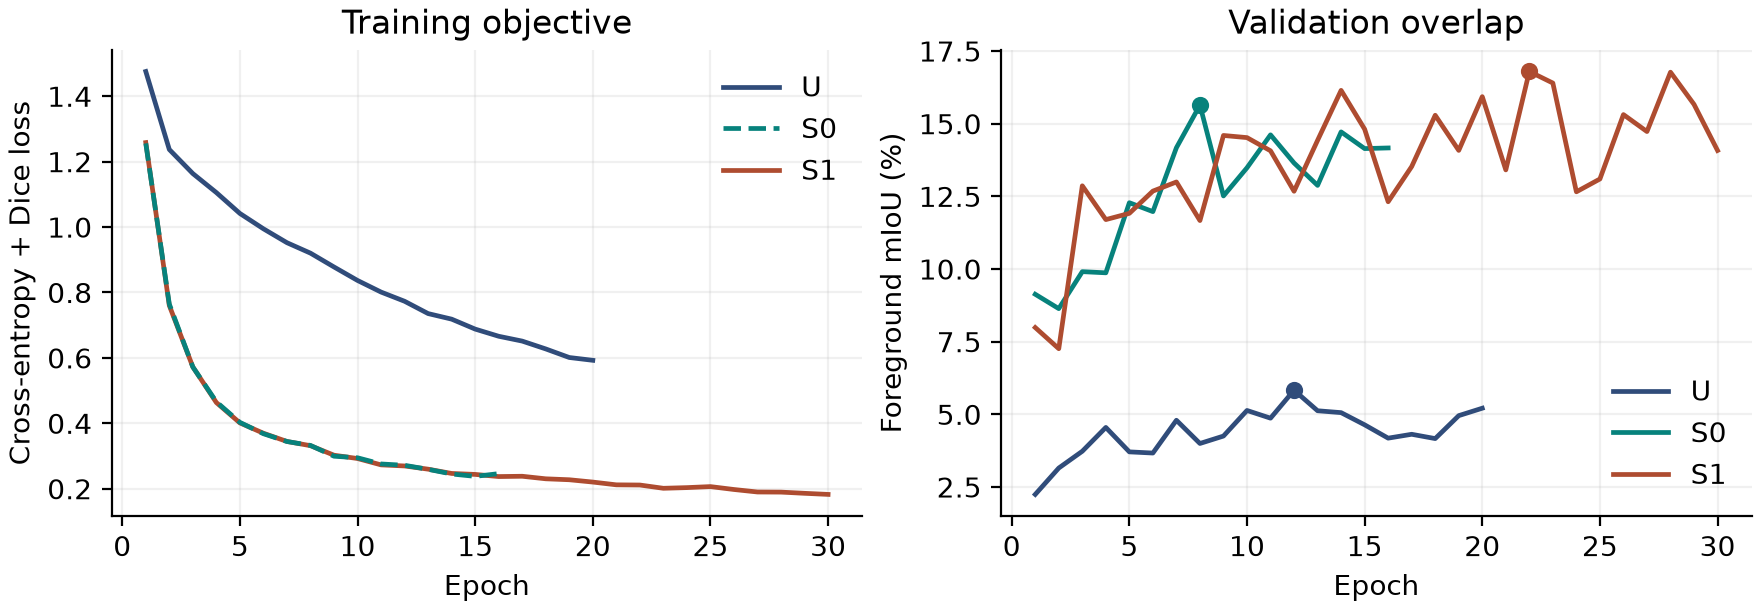
\includegraphics[width=\textwidth]{images/seed69_learning_curves.png}
\caption{Seed 69 training objective and validation FG mIoU. Dots mark validation-selected checkpoints.}\label{fig:final-curves}
\end{figure}
\begin{table}[H]\centering\small
\caption{Seed 69 compute cost. Train and validation hours sum the recorded phases through early stopping.}\label{tab:final-compute}
\begin{tabular}{@{}lrrrrr@{}}\toprule
Run & Parameters & Train (h) & Val (h) & Batch 4 (ms) & Amortized ms/image \\\midrule
U & 1,964,369 & 5.69 & 0.42 & 84.98 & 21.24 \\
S0 & 3,718,513 & 4.51 & 0.29 & 110.95 & 27.74 \\
S1 & 3,718,513 & 8.82 & 0.54 & 111.09 & 27.77 \\
\bottomrule
\end{tabular}
\end{table}

The forward benchmark uses a Tesla T4, FP32, a preloaded batch of four images, ten warm-ups and fifty timed forwards. Amortized time divides the median batch time by four. Data loading, transfers and postprocessing are excluded, so the timing describes the forward stage under this batch protocol. Appendix~\ref{app:curves} shows the loss and validation curves for all nine runs. At seed 69, S0 and S1 each stop eight epochs after their best checkpoint, so their different run lengths reflect the epoch of peak validation score.

\clearpage
\subsection{Class-level confusion on the held-out split}
Figure~\ref{fig:confusion} compares which labels the three configurations predict for each true class. For each seed we divide every confusion row by the number of valid ground-truth pixels in its class. Each cell then averages those percentages over the three seeds. Appendix~\ref{app:class} lists class IDs, IoU, Dice and pixel support.

\begin{figure}[H]\centering
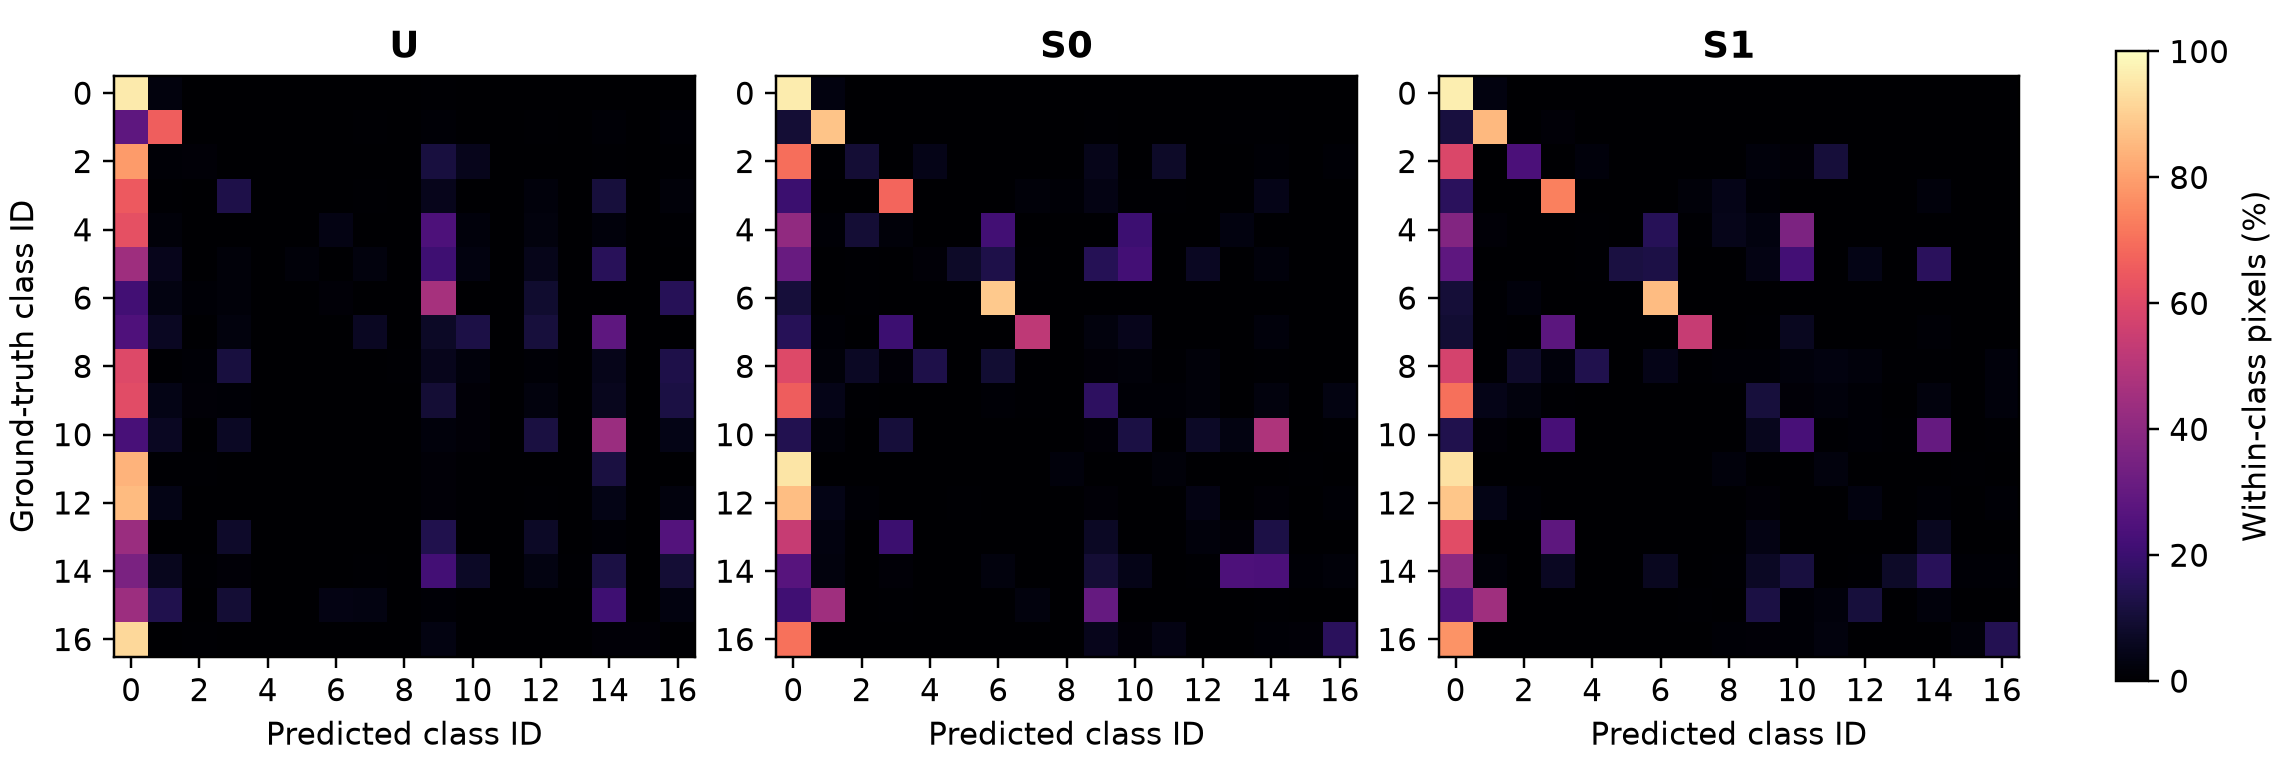
\includegraphics[width=\textwidth]{images/confusion_compact.png}
\caption{Test confusion by model using a common color scale. The first column is prediction as background. The diagonal gives the fraction of each ground-truth class labeled correctly.}\label{fig:confusion}
\end{figure}

The test matrices show that the mean share of true trash pixels predicted as background is 56.22\% for U, 52.76\% for S0 and 59.83\% for S1. S1 assigns more trash pixels to background than S0 at each seed, including seed 69 where S1 improves trash mIoU. These measures answer different questions. The background error weights pixels by their frequency and covers one prediction label, while trash mIoU gives the eight trash classes equal weight and accounts for false positives and false negatives. In the per-class comparison, augmentation increases mean IoU by 4.26 points for fabric and decreases it by 5.87 points for plastic.

\Needspace{20\baselineskip}
\subsection{Qualitative error analysis}
Figure~\ref{fig:final-errors} aligns the predictions of the three seed-69 checkpoints on three examples from the fixed gallery. The cases illustrate successes and failures. Whole-test counts below quantify one error type beyond the gallery.
\begin{figure}[H]\centering
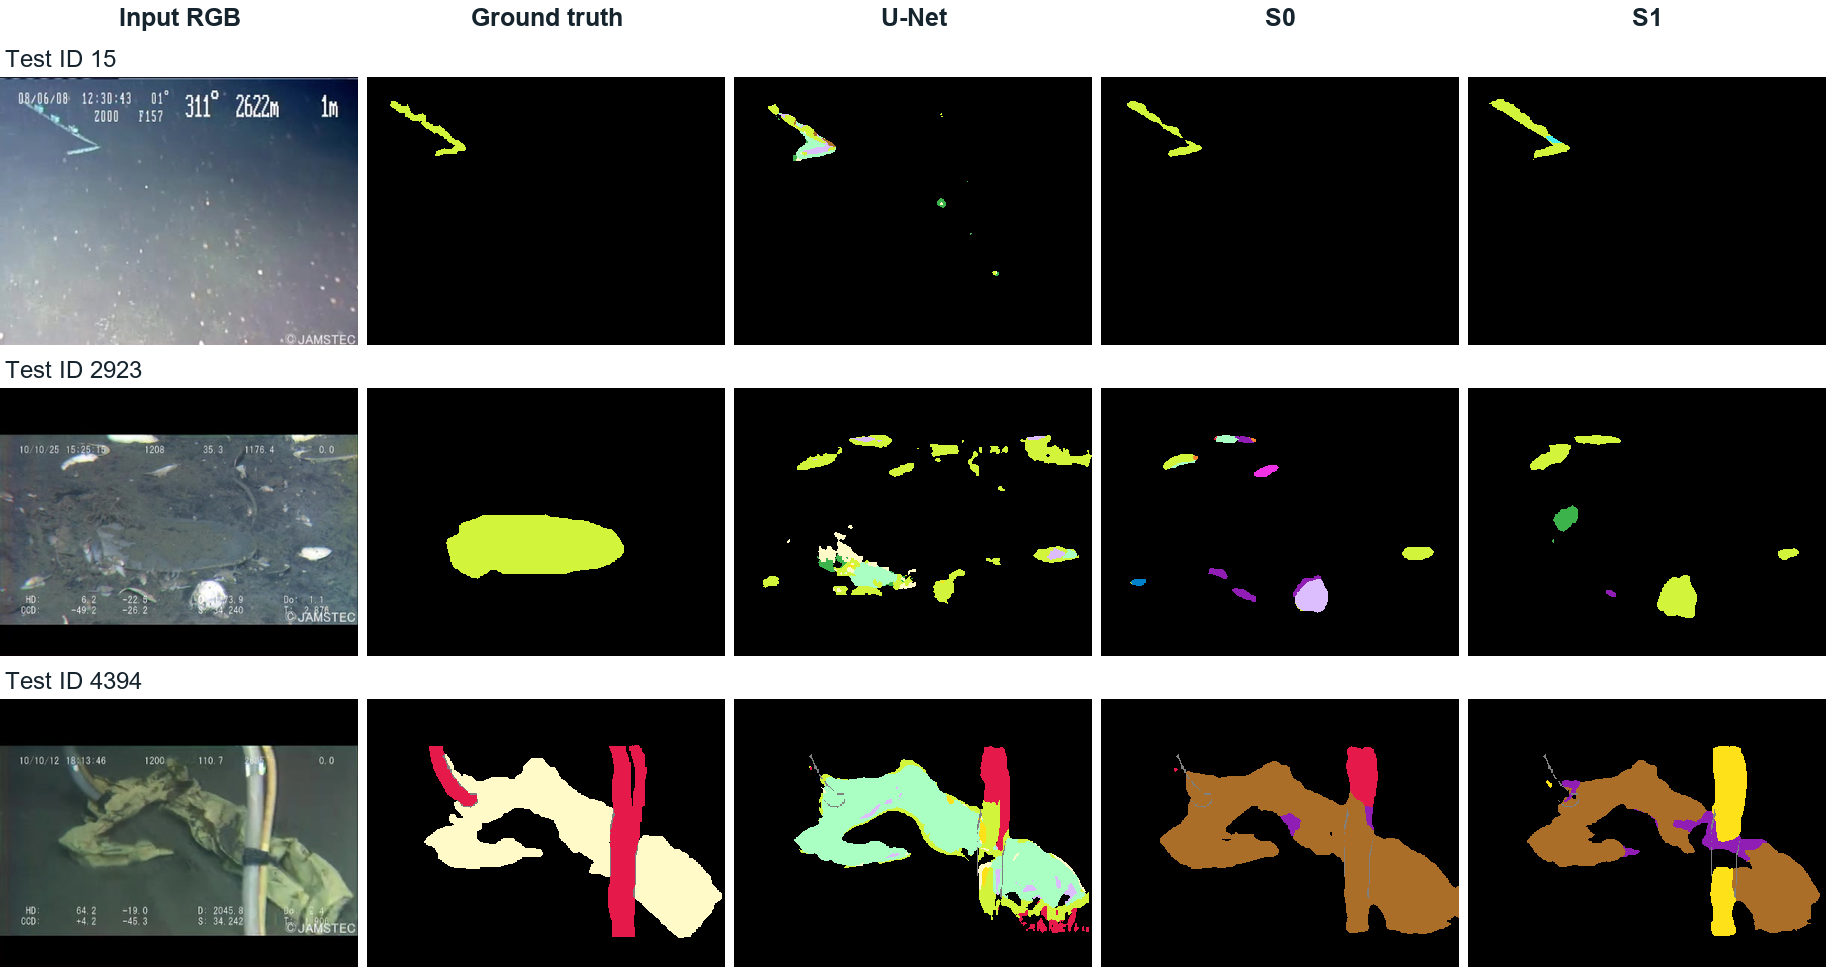
\includegraphics[width=\textwidth]{images/a2_seed69_error_cases.png}
\caption{Matched held-out cases. Columns show RGB, ground truth and predictions from U, S0 and S1. Row 1 shows a thin object, row 2 a foreground omission, and row 3 a material confusion. Vertical letterbox padding is cropped for display.}\label{fig:final-errors}
\end{figure}
On image 15, S1 assigns 1,299 of 1,527 true foreground pixels to the correct class, \texttt{trash\_etc}, against 1,095 for S0 and 664 for U. On image 2923, both SegFormer variants assign more than 98\% of the annotated foreground to background. On image 4394, both SegFormer variants localize much of the plastic region but label most of it as paper. This is a class confusion even when the foreground outline is approximately captured. Image contrast, class appearance and annotation boundaries are possible factors to examine with additional cases.

Over all held-out images at seed 69, the share of true foreground assigned to background is 43.8\% for U, 30.0\% for S0 and 35.2\% for S1. This measure uses the full confusion matrix and complements the visual examples.

\clearpage
\section{Limitations and conclusion}
The held-out evaluation uses one fixed split based on source video identifiers. Independence across dives and locations remains unverified. Rare classes and ignored cross-class conflicts limit what can be inferred from pixel overlap. U-Net is the smallest configuration and has the lowest observed forward cost at seed 69. Both SegFormer configurations give higher foreground and trash overlap in the measured tests. The selected augmentation does not show a consistent benefit across the three pairs. Further repeats in one execution environment and a test set from independent dives would better separate these effects.

\section{Reproducibility and evidence}
The companion LaTeX archive includes the exact source files covered by the run source digest, the split manifest, nine effective configs and histories, nine test outputs and completion records, available timing samples, and reproducibility notebooks. \path{REPRODUCIBILITY.md} gives environment settings, file layouts and commands.

\begin{enumerate}
\item \textbf{Check the report without retraining.} Run \path{python reproduction/verify_results.py} after extracting the source archive. The script uses only Python's standard library. It validates the test output hashes, recovers the selected epochs from the saved validation histories, and recomputes class overlap, three-seed summaries and paired differences.
\item \textbf{Check data preparation.} Obtain \path{dataset.zip} from the TrashCan dataset repository\cite{trashcandr} and extract the Material version. With the fixed manifest and Pillow 12.3.0, run \path{reproduction/make_example_batch.py} against that folder. Compare the IDs and mask hashes with \path{evidence/example_batch.json}.
\item \textbf{Repeat training or resume.} The fresh Kaggle notebook schedules all nine configurations. The historical continuation notebooks require the corresponding saved suite. Use the same split and accelerator profile, preserve the entire output root, and resume from the last completed epoch with \path{last.pt}. The run ID and checkpoint fingerprints distinguish reruns from the report's runs.
\item \textbf{Evaluate.} Use the validation-selected \path{best.pt} with the saved model config and the same test membership. The notebook produces \path{test_best.json}, \path{test_complete.json}, \path{test_confusion.csv} and \path{test_per_class.csv}. Use the reproduced metrics to compare protocol outcomes and keep the original test output available for review.
\end{enumerate}
The report audit checked 463 files from the 8 November export. Appendix~\ref{app:verify} records the U69 replay recovery and S1 continuation lineage. The full dataset and checkpoint binaries are kept separately from the report archive.

\section{Work allocation and AI-use disclosure}
The implementation plan assigned dataset and exploratory analysis to Nguyen Hao Thien, the shared training/evaluation engine and U-Net to Nguyen Anh Khoa, and SegFormer, reproducibility and integration to Ta Tuan Khai. These are planned areas of responsibility. The saved run artifacts describe the experiments without assigning individual authorship to each file.

OpenAI Codex assisted with code and notebook development, artifact verification, report organization, prose, figures and tables. The reported metrics come from project runs performed on Kaggle and Colab. The report audit and CPU batch reconstruction used the saved artifacts and pinned data adapter. The authors are responsible for checking the reported interpretation and confirming their contributions and AI-use disclosure before submission.

\Needspace{12\baselineskip}
\begin{thebibliography}{9}
\bibitem{trashcan} J. Hong, M. Fulton and J. Sattar. \emph{TrashCan: A Semantically-Segmented Dataset towards Visual Detection of Marine Debris}.2020. \url{https://arxiv.org/abs/2007.08097}.
\bibitem{trashcandr} M. S. Fulton, J. Hong and J. Sattar. \emph{TrashCan 1.0}. Data Repository for the University of Minnesota, 2020. \url{https://doi.org/10.13020/g1gx-y834}.
\bibitem{unet} O. Ronneberger, P. Fischer and T. Brox. \emph{U-Net: Convolutional Networks for Biomedical Image Segmentation}.2015. \url{https://arxiv.org/abs/1505.04597}.
\bibitem{segformer} E. Xie et al. \emph{SegFormer: Simple and Efficient Design for Semantic Segmentation with Transformers}.2021. \url{https://arxiv.org/abs/2105.15203}.
\bibitem{segformerconfig} NVIDIA. \emph{SegFormer-B0 ADE20K 512 checkpoint configuration}, revision \cls{489d5cd}. \url{https://huggingface.co/nvidia/segformer-b0-finetuned-ade-512-512/blob/489d5cd81a0b59fab9b7ea758d3548ebe99677da/config.json}.
\bibitem{project} Tiki-taka. \emph{TrashCan-Material EDA, fixed seed 36 manifest, source snapshots, setup/pilot ledgers and run artifacts}. EDA measured 5 October 2026; training artifacts audited through 8 November 2026. Machine-readable evidence accompanies this report source.
\end{thebibliography}

\clearpage
\appendix
\section{Effective configurations and architectures}
\label{app:config}
Table~\ref{tab:full-config} records the settings that distinguish the three configurations. All nine effective JSON snapshots are provided in \path{evidence/runs/}. A paired S0/S1 run changes only the color-jitter switch in the model and training design. The frozen pilot reference and run name identify each execution.

\begin{table}[H]\centering\small
\caption{Effective experiment settings. Trainable counts exclude buffers.}\label{tab:full-config}
\begin{tabularx}{\linewidth}{@{}lYYY@{}}\toprule
Setting & U & S0 & S1 \\ \midrule
Architecture & Compact U-Net & SegFormer-B0 & SegFormer-B0 \\
Initialization & Scratch & ADE20K pretrained with new head & Same per-seed state as S0 \\
Trainable / frozen & 1,964,369 / 0 & 3,718,513 / 0 & 3,718,513 / 0 \\
Learning rate & $10^{-3}$ & $6\times10^{-5}$ & $6\times10^{-5}$ \\
Training color jitter & Off & Off & On with probability 0.5 \\
Output classes & 17 & 17 & 17 \\ \bottomrule
\end{tabularx}
\end{table}

The shared budget uses AdamW with weight decay 0.01, batch size 4, up to 40 epochs, patience 8, full 32-bit precision, no scheduler and disabled TF32. The target uses ignore 255 and the loss is CE plus soft Dice with weights 1 and 1. Source and preprocessing are checked against the fixed split manifest before a run. The loader uses zero workers in the recorded run protocol.

The U-Net encoder channels are 16, 32, 64, 128 and 256. Each double-convolution block uses $3\times3$ convolutions, GroupNorm with eight groups and ReLU. The upsampling path concatenates skip features and uses the same block type. The SegFormer encoder has four stages with widths 32, 64, 160 and 256, attention heads 1, 2, 5 and 8, and spatial-reduction ratios 8, 4, 2 and 1\cite{segformerconfig}. The decoder projects each stage to width 256 and uses an aligned fusion head.

\clearpage
\section{Per-seed results and run provenance}
\label{app:runs}
\begingroup
\setstretch{1.06}
\setlength{\intextsep}{7pt}
Table~\ref{tab:final-seed-results} reports the held-out scores. Table~\ref{tab:validation-best} reports validation metrics at the epochs selected for test.

\begin{table}[H]\centering\small
\caption{Selected validation checkpoints. The three overlap columns are percentages.}\label{tab:validation-best}
\begin{tabular}{@{}rlrrrrr@{}}\toprule
Seed & Run & Best epoch & FG mIoU & FG Dice & Trash mIoU & Loss \\ \midrule
69420 & U & 15 & 5.309 & 8.437 & 3.270 & 1.3902 \\
69420 & S0 & 15 & 19.534 & 28.051 & 13.787 & 1.1341 \\
69420 & S1 & 14 & 17.580 & 25.876 & 11.361 & 1.1386 \\
67 & U & 15 & 6.137 & 9.130 & 3.611 & 1.3118 \\
67 & S0 & 20 & 19.125 & 27.528 & 13.133 & 1.0426 \\
67 & S1 & 9 & 16.994 & 25.014 & 13.954 & 1.0869 \\
69 & U & 12 & 5.830 & 8.923 & 3.427 & 1.2957 \\
69 & S0 & 8 & 15.639 & 23.365 & 12.321 & 1.0800 \\
69 & S1 & 22 & 16.796 & 25.283 & 14.292 & 1.2067 \\
\bottomrule\end{tabular}

\end{table}

Table~\ref{tab:provenance} maps the score rows to their checkpoints. See \path{verified_results.json} for full IDs and hashes.
\begin{table}[H]\centering\small
\caption{Active run identifier and evaluated checkpoint fingerprint for each result.}\label{tab:provenance}
\begin{tabular}{@{}rllll@{}}\toprule
Seed & Run & Platform & Run ID prefix & Checkpoint SHA prefix \\ \midrule
69420 & U & Colab & \cls{59a5534d} & \cls{05aa0e8acf65} \\
69420 & S0 & Colab & \cls{44b2f727} & \cls{1dfcd83afce2} \\
69420 & S1 & Colab & \cls{9d2434a5} & \cls{5d6070706d75} \\
67 & U & Kaggle & \cls{520488aa} & \cls{cf6df95b2a78} \\
67 & S0 & Kaggle $\to$ Colab & \cls{73460d50} & \cls{aa669fc9ae93} \\
67 & S1 & Colab & \cls{5bbb6140} & \cls{08fbda83ed36} \\
69 & U & Colab & \cls{d11fd7e4} & \cls{aaf72e433d33} \\
69 & S0 & Colab & \cls{7c6af03c} & \cls{64f1f8cf41ed} \\
69 & S1 & Colab & \cls{c6cef0a6} & \cls{2c2868ab7113} \\
\bottomrule\end{tabular}

\end{table}

\begin{table}[H]\centering\small
\caption{S1 minus S0 validation deltas in percentage points and outcome of the proposal rule. The held-out deltas appear separately in Table~\ref{tab:final-paired-deltas}.}\label{tab:validation-deltas}
\begin{tabular}{@{}rrrrl@{}}\toprule
Seed & FG mIoU & FG Dice & Trash mIoU & Rule \\ \midrule
69420 & -1.953 & -2.175 & -2.425 & Not met \\
67 & -2.131 & -2.515 & +0.821 & Not met \\
69 & +1.157 & +1.917 & +1.971 & Met \\
\bottomrule\end{tabular}

\end{table}
\endgroup

\clearpage
\section{Additional class-level results}
\label{app:class}
The class means and sample standard deviations in Tables~\ref{tab:class-iou} and \ref{tab:class-dice} use the three repeated evaluations of the same 1,078 test images. Pixel support counts each test pixel once. All 17 classes have nonzero target support. The final column of Table~\ref{tab:class-iou} is the mean of the three paired seed differences in IoU.

\begin{table}[H]\centering\footnotesize
\caption{Held-out per-class IoU, mean $\pm$ sample SD (\%). S1--S0 is in percentage points.}\label{tab:class-iou}
\begin{tabular}{@{}rlrrrrr@{}}\toprule
ID & Class & Test pixels & U & S0 & S1 & S1--S0 (pp) \\ \midrule
0 & \cls{background} & 168,351,826 & $91.33\pm 0.32$ & $93.36\pm 0.15$ & $93.14\pm 0.10$ & -0.22 \\
1 & \cls{rov} & 7,661,326 & $41.00\pm 5.30$ & $52.82\pm 0.66$ & $52.06\pm 1.04$ & -0.77 \\
2 & \cls{plant} & 752,406 & $0.94\pm 0.58$ & $8.59\pm 3.89$ & $16.62\pm 14.49$ & +8.03 \\
3 & \cls{animal_fish} & 1,793,990 & $10.75\pm 6.14$ & $60.94\pm 14.22$ & $56.54\pm 1.50$ & -4.40 \\
4 & \cls{animal_starfish} & 25,521 & $0.13\pm 0.23$ & $0.04\pm 0.06$ & $0.18\pm 0.21$ & +0.14 \\
5 & \cls{animal_shells} & 6,789 & $0.72\pm 1.24$ & $2.44\pm 1.63$ & $3.76\pm 0.75$ & +1.32 \\
6 & \cls{animal_crab} & 223,331 & $0.97\pm 1.68$ & $46.26\pm 12.25$ & $41.97\pm 13.81$ & -4.30 \\
7 & \cls{animal_eel} & 87,276 & $3.02\pm 1.86$ & $29.55\pm 10.20$ & $27.76\pm 6.29$ & -1.80 \\
8 & \cls{animal_etc} & 201,098 & $0.43\pm 0.72$ & $0.26\pm 0.39$ & $0.71\pm 1.19$ & +0.44 \\
9 & \cls{trash_etc} & 1,822,549 & $4.72\pm 1.46$ & $11.34\pm 4.90$ & $8.00\pm 7.03$ & -3.34 \\
10 & \cls{trash_fabric} & 400,513 & $0.50\pm 0.83$ & $6.72\pm 5.81$ & $10.98\pm 0.75$ & +4.26 \\
11 & \cls{trash_fishing_gear} & 244,584 & $0.00\pm 0.00$ & $0.77\pm 0.35$ & $0.84\pm 1.46$ & +0.08 \\
12 & \cls{trash_metal} & 1,450,361 & $0.49\pm 0.54$ & $3.31\pm 1.04$ & $2.80\pm 0.81$ & -0.50 \\
13 & \cls{trash_paper} & 63,828 & $0.00\pm 0.00$ & $0.14\pm 0.24$ & $0.00\pm 0.00$ & -0.14 \\
14 & \cls{trash_plastic} & 2,822,298 & $8.53\pm 1.76$ & $19.72\pm 8.54$ & $13.85\pm 4.21$ & -5.87 \\
15 & \cls{trash_rubber} & 53,751 & $0.01\pm 0.02$ & $0.00\pm 0.00$ & $0.02\pm 0.04$ & +0.02 \\
16 & \cls{trash_wood} & 378,513 & $0.10\pm 0.17$ & $10.78\pm 5.84$ & $10.54\pm 2.75$ & -0.24 \\
\bottomrule\end{tabular}

\end{table}
Plastic has the largest IoU decline among trash classes in the paired means. Paper and rubber have low IoU across configurations, and have substantially fewer test pixels than plastic.

\begin{table}[H]\centering\footnotesize
\caption{Held-out per-class Dice, mean $\pm$ sample SD (\%).}\label{tab:class-dice}
\begin{tabular}{@{}rlrrrr@{}}\toprule
ID & Class & Test pixels & U & S0 & S1 \\ \midrule
0 & \cls{background} & 168,351,826 & $95.47\pm 0.17$ & $96.57\pm 0.08$ & $96.45\pm 0.06$ \\
1 & \cls{rov} & 7,661,326 & $58.02\pm 5.35$ & $69.13\pm 0.57$ & $68.46\pm 0.90$ \\
2 & \cls{plant} & 752,406 & $1.86\pm 1.15$ & $15.67\pm 6.55$ & $26.75\pm 21.27$ \\
3 & \cls{animal_fish} & 1,793,990 & $19.03\pm 10.36$ & $75.07\pm 11.14$ & $72.23\pm 1.23$ \\
4 & \cls{animal_starfish} & 25,521 & $0.27\pm 0.45$ & $0.08\pm 0.13$ & $0.35\pm 0.43$ \\
5 & \cls{animal_shells} & 6,789 & $1.40\pm 2.43$ & $4.74\pm 3.08$ & $7.25\pm 1.38$ \\
6 & \cls{animal_crab} & 223,331 & $1.89\pm 3.27$ & $62.65\pm 10.97$ & $58.26\pm 13.30$ \\
7 & \cls{animal_eel} & 87,276 & $5.82\pm 3.49$ & $45.00\pm 11.87$ & $43.20\pm 7.72$ \\
8 & \cls{animal_etc} & 201,098 & $0.85\pm 1.41$ & $0.53\pm 0.78$ & $1.39\pm 2.33$ \\
9 & \cls{trash_etc} & 1,822,549 & $8.99\pm 2.67$ & $20.14\pm 8.09$ & $14.31\pm 11.67$ \\
10 & \cls{trash_fabric} & 400,513 & $0.98\pm 1.63$ & $12.24\pm 10.08$ & $19.78\pm 1.22$ \\
11 & \cls{trash_fishing_gear} & 244,584 & $0.00\pm 0.00$ & $1.52\pm 0.70$ & $1.64\pm 2.84$ \\
12 & \cls{trash_metal} & 1,450,361 & $0.97\pm 1.07$ & $6.39\pm 1.97$ & $5.44\pm 1.54$ \\
13 & \cls{trash_paper} & 63,828 & $0.00\pm 0.00$ & $0.28\pm 0.48$ & $0.00\pm 0.00$ \\
14 & \cls{trash_plastic} & 2,822,298 & $15.69\pm 3.00$ & $32.38\pm 11.81$ & $24.17\pm 6.42$ \\
15 & \cls{trash_rubber} & 53,751 & $0.03\pm 0.04$ & $0.00\pm 0.00$ & $0.05\pm 0.08$ \\
16 & \cls{trash_wood} & 378,513 & $0.19\pm 0.33$ & $19.13\pm 9.29$ & $18.99\pm 4.44$ \\
\bottomrule\end{tabular}

\end{table}
Dice shows the same broad class-level difficulties. The bundled per-run confusion matrices retain the exact counts behind both measures.

\begin{table}[H]\centering\small
\caption{Percentage of true foreground or trash pixels assigned to background, by seed and model.}\label{tab:appendix-background}
\begin{tabular}{@{}rrrrrrr@{}}\toprule
Seed & U FG & S0 FG & S1 FG & U trash & S0 trash & S1 trash \\ \midrule
69420 & 51.00 & 34.43 & 33.24 & 62.50 & 57.43 & 60.25 \\
67 & 42.88 & 29.41 & 33.56 & 53.04 & 50.84 & 60.91 \\
69 & 43.77 & 30.01 & 35.22 & 53.12 & 50.01 & 58.31 \\
\bottomrule\end{tabular}

\end{table}
Every row shows a higher trash-to-background rate for S1 than for S0, despite the different directions of the trash mIoU changes. The CSV also provides the pixel numerators and denominators.

\clearpage
\section{Training histories for all nine runs}
\label{app:curves}
Figure~\ref{fig:all-curves} shows the saved epoch histories underlying the best-epoch and early-stopping results. Each row uses a common x-axis and each metric uses the same y-scale across seeds. Dots mark the epochs evaluated on test.
\begin{figure}[H]\centering
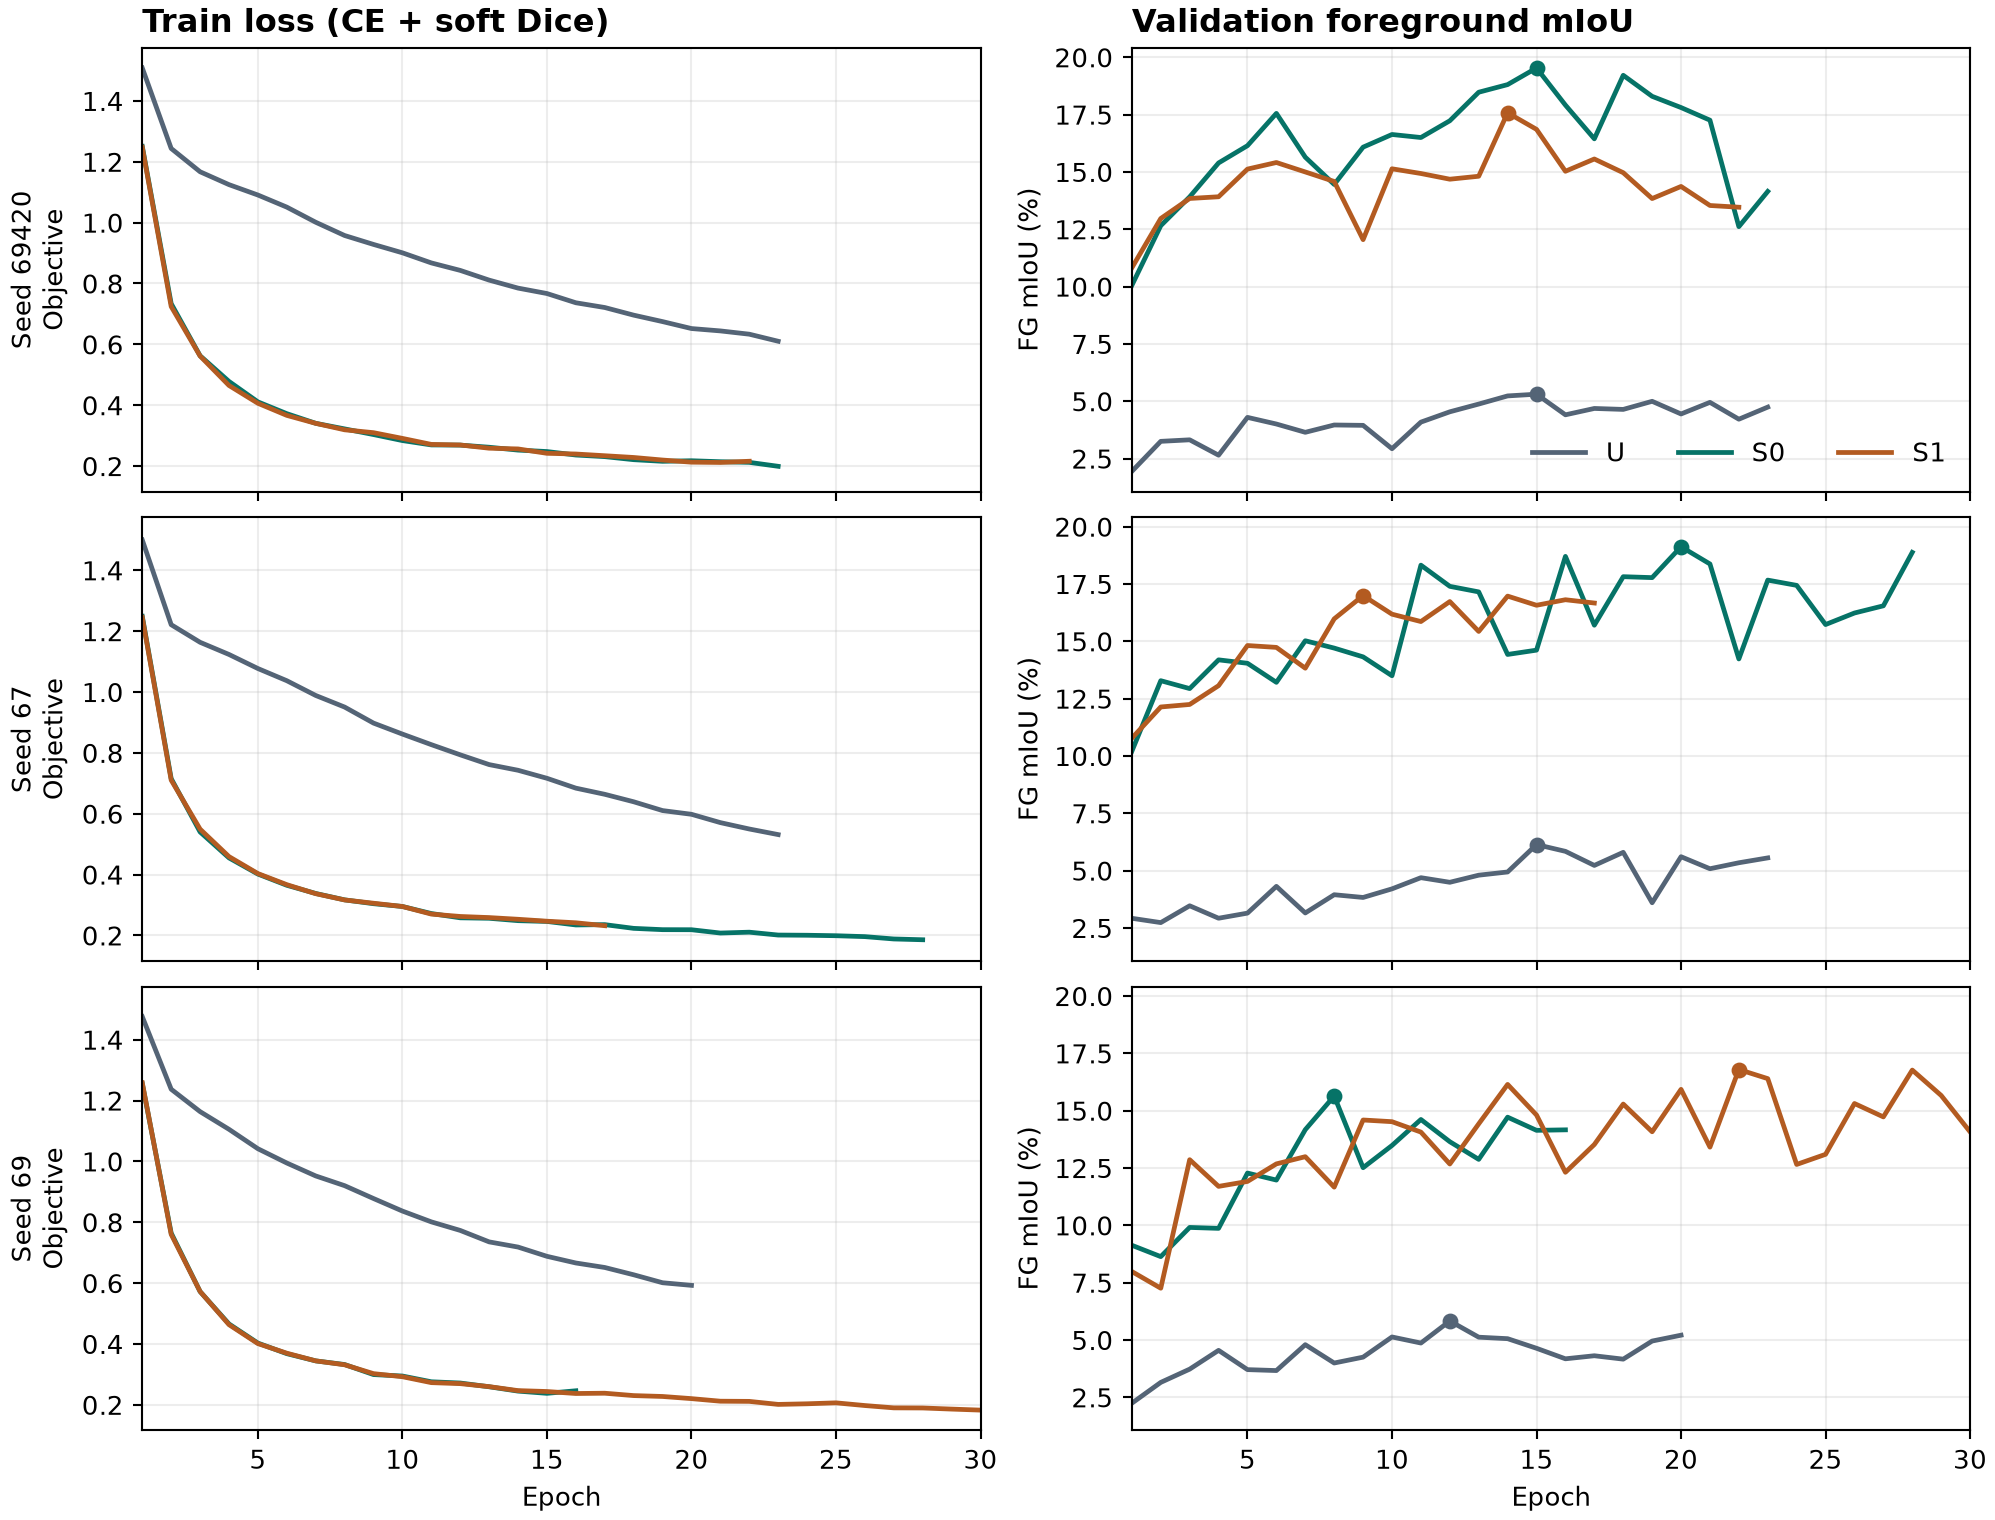
\includegraphics[width=\textwidth]{images/all_seed_curves.png}
\caption{Train objective and validation foreground mIoU for U, S0 and S1 across all seeds. Curves stop at the last completed epoch.}\label{fig:all-curves}
\end{figure}
Both SegFormer configurations reach higher validation foreground mIoU than U at every seed. The differing peak positions explain why early stopping runs for different numbers of epochs under the same patience.

\clearpage
\section{Verification and continuation notes}
\label{app:verify}
The source revision and common dataset identities are listed below. The archive SHA-256 hashes the raw ZIP bytes. The manifest digest hashes its canonical content. The test membership digest binds the ordered test rows.
\begin{description}
\item[Source revision] \path{7df323698d1ae4d5122850a54eb38b01609d80f1}
\item[Archive SHA-256] \path{caf93d992b85343cfc500386c94ca9ffa6c63e2284e04127753a40db8f33ba4c}
\item[Manifest content digest] \path{87905f1a97dd2c04194e049ca61d1a7f3bbe2942e9fe17dc2d737c371cdce943}
\item[Test membership digest] \path{738b95e533e0dc479c247f5a0c62d1298dec6a0d15cc65b88a71b689f1c7e147}
\end{description}

The 8 November audit checked export hashes, test/checkpoint and membership binding, history order, validation checkpoint selection and per-class metrics. The nine test outputs each contain 186,339,960 valid pixels after excluding ignore and padding. Raw test results come from the recorded GPU inference runs. The packaged verifier recomputes metrics from those saved counts.

Table~\ref{tab:continuation} records three execution paths that require care when reading the results.
\begin{table}[H]\centering\small
\caption{Continuation and replay evidence. Epochs count within the same experiment.}\label{tab:continuation}
\begin{tabularx}{\linewidth}{@{}lYY@{}}\toprule
Run & Recorded event & Evidence treatment \\ \midrule
S0, seed 67 & Resumed after epoch 7 from Kaggle on Colab and finished at epoch 28. & Retains the common history prefix and seed. Labeled as a mixed runtime. \\
U, seed 69 & Training ended at epoch 20. Replay of the epoch-12 validation checkpoint changed nine confusion cells. & Half the absolute count difference was five of 176,765,049 valid pixels. The narrow replay receipt is bound to the audited artifacts. Test evaluates the original best checkpoint. \\
S1, seed 69 & Continued after epochs 21 and 28. Finished at epoch 30 with best epoch 22. & Parent checkpoint hashes and history prefixes preserve one experiment across resumes. \\
\bottomrule\end{tabularx}
\end{table}
The retained validation replay receipt and available raw T4 timing logs are included under the relevant run folders. Model state and optimizer/RNG state are stored separately in the original checkpoint archives. Exact continuation depends on those archives and their numerical runtime settings.

\end{document}
